\documentclass[english]{article}
\usepackage{amsmath}
\usepackage{ae,aecompl}
\usepackage[T1]{fontenc}
\usepackage[latin9]{inputenc}
\usepackage{textcomp}
\usepackage{graphicx}
\usepackage{eurosym}
\usepackage[hidelinks]{hyperref}
\usepackage{float}
\usepackage{fancyhdr}
\usepackage{tabto}
\usepackage{verbatim}
\usepackage{etoolbox}
\usepackage[table]{xcolor}
\usepackage{booktabs}
\usepackage{wasysym}
\usepackage{multirow}
\usepackage{fancyhdr}
\usepackage{pdflscape}
\usepackage[scaled]{beramono}
\usepackage{listings}
\lstset{
  language=Python,
  showstringspaces=false,
  stringstyle = \color{mymauve},
  formfeed=\newpage,
  tabsize=4,
  commentstyle=\itshape,
  basicstyle=\ttfamily,
    numbers=left,
    stepnumber=1,
    numbersep=6pt,
    numberblanklines=false,
    numberstyle=\tiny\bf,
    keywordstyle=\color{blue},
    commentstyle=\color{mygreen},
    identifierstyle==\color{orange},
}
\definecolor{mygreen}{rgb}{0,0.6,0}
\definecolor{mygray}{rgb}{0.5,0.5,0.5}
\definecolor{mymauve}{rgb}{0.58,0,0.82} 

\newcommand{\code}[2]{
  \hrulefill
  \subsection*{#1}
  \lstinputlisting{#2}
  \vspace{2em}
}

\pagestyle{fancy}
\lhead{\powerenjoy Design Document}
\makeatletter
\makeatother
\usepackage{babel}

\newcommand\fnurl[2]{%
	\href{#2}{#1}\footnote{\url{#2}}%
}
\newcommand{\rent}{\textit{rent }}
\newcommand{\carsharing}{\textit {car sharing }}
\newcommand{\powerenjoy}{\textit{PowerEnjoy }}
\newcommand{\registereduser}{\textit {registered user }}
\newcommand{\registeredusers}{\textit {registered users }}
\newcommand{\powerenjoyuser}{\textit{PowerEnjoy User }}
\newcommand{\staff}{\textit{staff }}
\newcommand{\service}{\textit{service }}
\newcommand{\services }{\textit{services }}
\newcommand{\safearea}{\textit{safe area }}
\newcommand{\safeareas}{\textit{safe areas }}
\newcommand{\powerplug}{\textit{power plug }}
\newcommand{\powerplugs}{\textit{power plugs }}
\newcommand{\reservation}{\textit{reservation }}
\newcommand{\stand}{\textit{stand }}
\newcommand{\fieldstaff}{\textit{field staff }}
\newcommand{\resevation}{\textit{reservation }}
\newcommand{\stopover}{\textit{stopover }}
\newcommand{\personalpin}{\textit{personal pin }}
\newcommand{\guest}{\textit{guest }}
\newcommand{\thirdparty}{\textit{third party developer }}
\newcommand{\powerplugslot}{\textit{power plug slot }}
\newcommand{\moneysaving}{\textit{money saving }}
\begin{document}

	\begin{figure}
		\centering
		
\includegraphics[scale=0.5]{logo.pdf} 
	\end{figure}


	\title{PowerEnJoy\\
	Design Document\\
	}

	\date{A.A 2016/2017}
	
	\author{Erba Alessandro\\
	 Leveni Filippo\\
	 Lodi Luca}
	
	\maketitle
	\pagebreak{}

\tableofcontents{} \pagebreak{}
\section{Introduction}
	\subsection{Purpose}
		In the RASD document we have presented the objectives and a general overview of PowerEnjoy system.
		The purpose of this document is to give more technical details about software and hardware choices that we have found for the system realization.
		However our main focus will be on software design, because this document will provide the fundamental specifications that will allow the developers to implement the application.
	\subsection{Scope}
		In order to best describe the architecture and the runtime view of the application, we are going to use different type of diagrams. Such diagrams should convey as much as possible the information on how the software is going to be structured.
		In particular we will present some UML diagrams:
			\begin{itemize}
				\item{Component Diagram, to describe the high and the low level of the software's architectural structure}
				\item{Deployment Diagram, to describe the hardware's architectural structure and how the software is mapped on it}
				\item{Sequence Diagram, to describe the behavior at runtime of the software}
			\end{itemize}
		 We will specify which architectural pattern we have chosen and how they are used, we will give a description of the most crucial algorithms and a description of the user interface. Finally, for sake of completeness, we will show how every requirement defined in the RASD document is mapped in this document.
	\subsection{Definitions, Acronyms, Abbreviations}
		\subsubsection{Rent}
			A \rent is the activity beginning with the pick up and ending with the release of a car. It can include some \stopover.
		\subsubsection{Car Sharing}
			\carsharing is a model of car rental where people rent cars for short periods of time, often by the hour.
		\subsubsection{PowerEnJoy}
			\powerenjoy is the \carsharing brand object of this document.
		\subsubsection{Guest User}
			A \guest is a person not logged in to the system.
		\subsubsection{Registered User} 
			A \registereduser is a person registered to \powerenjoy.
		\subsubsection{PowerEnJoy User}
			A \powerenjoyuser is a \registereduser can access to the \carsharing through his smart device.
		\subsubsection{Staff}
			\staff is the set of people that are \registereduser  but can perform special operations. They are divided in three different categories.
			\begin{itemize}
				\item {Field \staff}
				\begin{itemize}
				\item They own a passepartout for cars reporting any issues \\ \par (e.g: cars with low battery).
				\end{itemize}
				\item{Emergency \staff}
				\begin{itemize}
				\item They manage users issues. They are able to directly contact users.
				\end{itemize}
				\item{Management \staff}
				\begin{itemize}
				\item They manage the system, configuring its parameters. They can add new \safeareas, modify \carsharing fares and create new \staff accounts.
				\end{itemize}
			\end{itemize}
		\subsubsection{Third Party Developer}
			\thirdparty is a person that can fulfill operations on \powerenjoy system via API.
		\subsubsection{Service}
			The \service is the group of actions that a \powerenjoyuser can fulfill trough his smart device.	
		\subsubsection {Safe Area}
			A \safearea is a  geographical place\footnote{defined by a set of geolocation positions} on the map in which parking is allowed. \safearea are saved into the system. A \rent can end parking the car only in safe areas.
	\subsubsection{Power Plug}
		A \powerplug is the station that charges the battery of an electric car. All \powerplugs are displayed in the map on-board \powerenjoy cars. Each \powerplug is in a \safearea. A \powerenjoyuser who plugs his car into a \powerplug receives a discount according to \powerenjoy rules.
	\subsubsection{Power Plug Slot}
		A \powerplugslot is a parking slot reserved for the \powerplug charge of cars.
	\subsubsection{Parking solution}
		Either a \safearea or a \powerplugslot.
	\subsubsection{Reservation}
		A \resevation is the action of booking a car, within an hour from its pick up.
	\subsubsection{Stopover}
		A \stopover is a temporary power-off of a rented car. During a \stopover the \powerenjoyuser can leave the car,  and re-unlock it later through his smart device. It is subject to a different fare than the rest of rent time.
	\subsubsection{Fare}
		A policy to compute price of a rent, complete of involved parameters. \par E.g: proportional to time, 0.67\euro/minute during active rent time 
	\subsubsection{Personal Identification Number (PIN)}
		 \personalpin is a number of 5 digits that the user inserts on the car screen to enable driving commands.
	\subsection{Reference Documents}
		\begin{itemize}
			\item{AssignmentsAA2016-2017.pdf for the index. It can be retrieved on beep.}
			\item{RASD.pdf for all the not-architectural choices. In can be retrieved on GitHub.}
		\end{itemize}
	\subsection{Document Structure}
		The document will be divided in 7 sections:
			\begin{enumerate}
				\item{Introduction: A brief description of the content and the purpose of the document}
				\item{Architectural Design: This will be the main section of the document and will provide the design of the application. It will contains all the UML diagrams needed to specify how the software is going to be implemented (thus, the software design) and the architectural choices made in the design process.}
				\item{Algorithm Design: This section will provide an insight on how the most crucial and important algorithms of our application will work.}
				\item{User Interface Design: This section will provide a point of view over the design of the user interface. This has already been aleady discussed in the RASD through some mockups, however in this document will provide a more complete explanation of the user interface.}
				\item{Requirements Traceability: In this section we will provide the mapping between the requirements identified in the RASD and our design decisions.}
				\item{Effort Spent: Here we will indicate hours spent by each members of the group to carry out this document.}
				\item{References: This section groups all links that refers to external material which was useful in the document writing.}
			\end{enumerate}
\section{Architectural Design}
	\subsection{Overview}%High level components and their interaction
				The system is split over a server and five client applications, for Cars,  PowerEnJoy users, Field Staff users, Emergency Staff users and Management Staff users respectively.\\
		The server  run business logic such as rent and reservation management, execute BPM and communicate with car's software to monitor eventual emergencies.
		The server relies on an external DBMS for data persistence, and multiple server instances are organized by a load balancer.\\
		The PowerEnJoy app interface the service's user with the back-end system in order  to register, to perform rents and reservations and to be updated of change in the terms of service. In addition it regularly update the user position's information in the back-end. \\
		Field Staff application is responsible of displaying incoming relocation and maintenance requests. It also contains information to quickly contact emergency support. \\
		Car's application is designed to handle the car-related steps of rent experience, providing remote data acquisition and actuators control capability to the back-end system.
		It regularly update the car position's information on the back-end, and enable the user to perform money saving option. Moreover it receives updates for the navigation system (such as new PowerPlug slots' or SafeArea's locations). \\
		Emergency Staff application provide an overview over all main service's informations to the corresponding staff and empower them with the tools to handle almost every possible emergency situation (cancel rents or reservations, assign relocation/maintenance requests, ...).  The app shows the information about the assigned emergency tasks for the app-user. \\
		Management Staff users can update and configure almost every service parameter by their application, from fares and discounts to term of services and SafeAreas' locations.
			\begin{figure}[H]
				\centering
				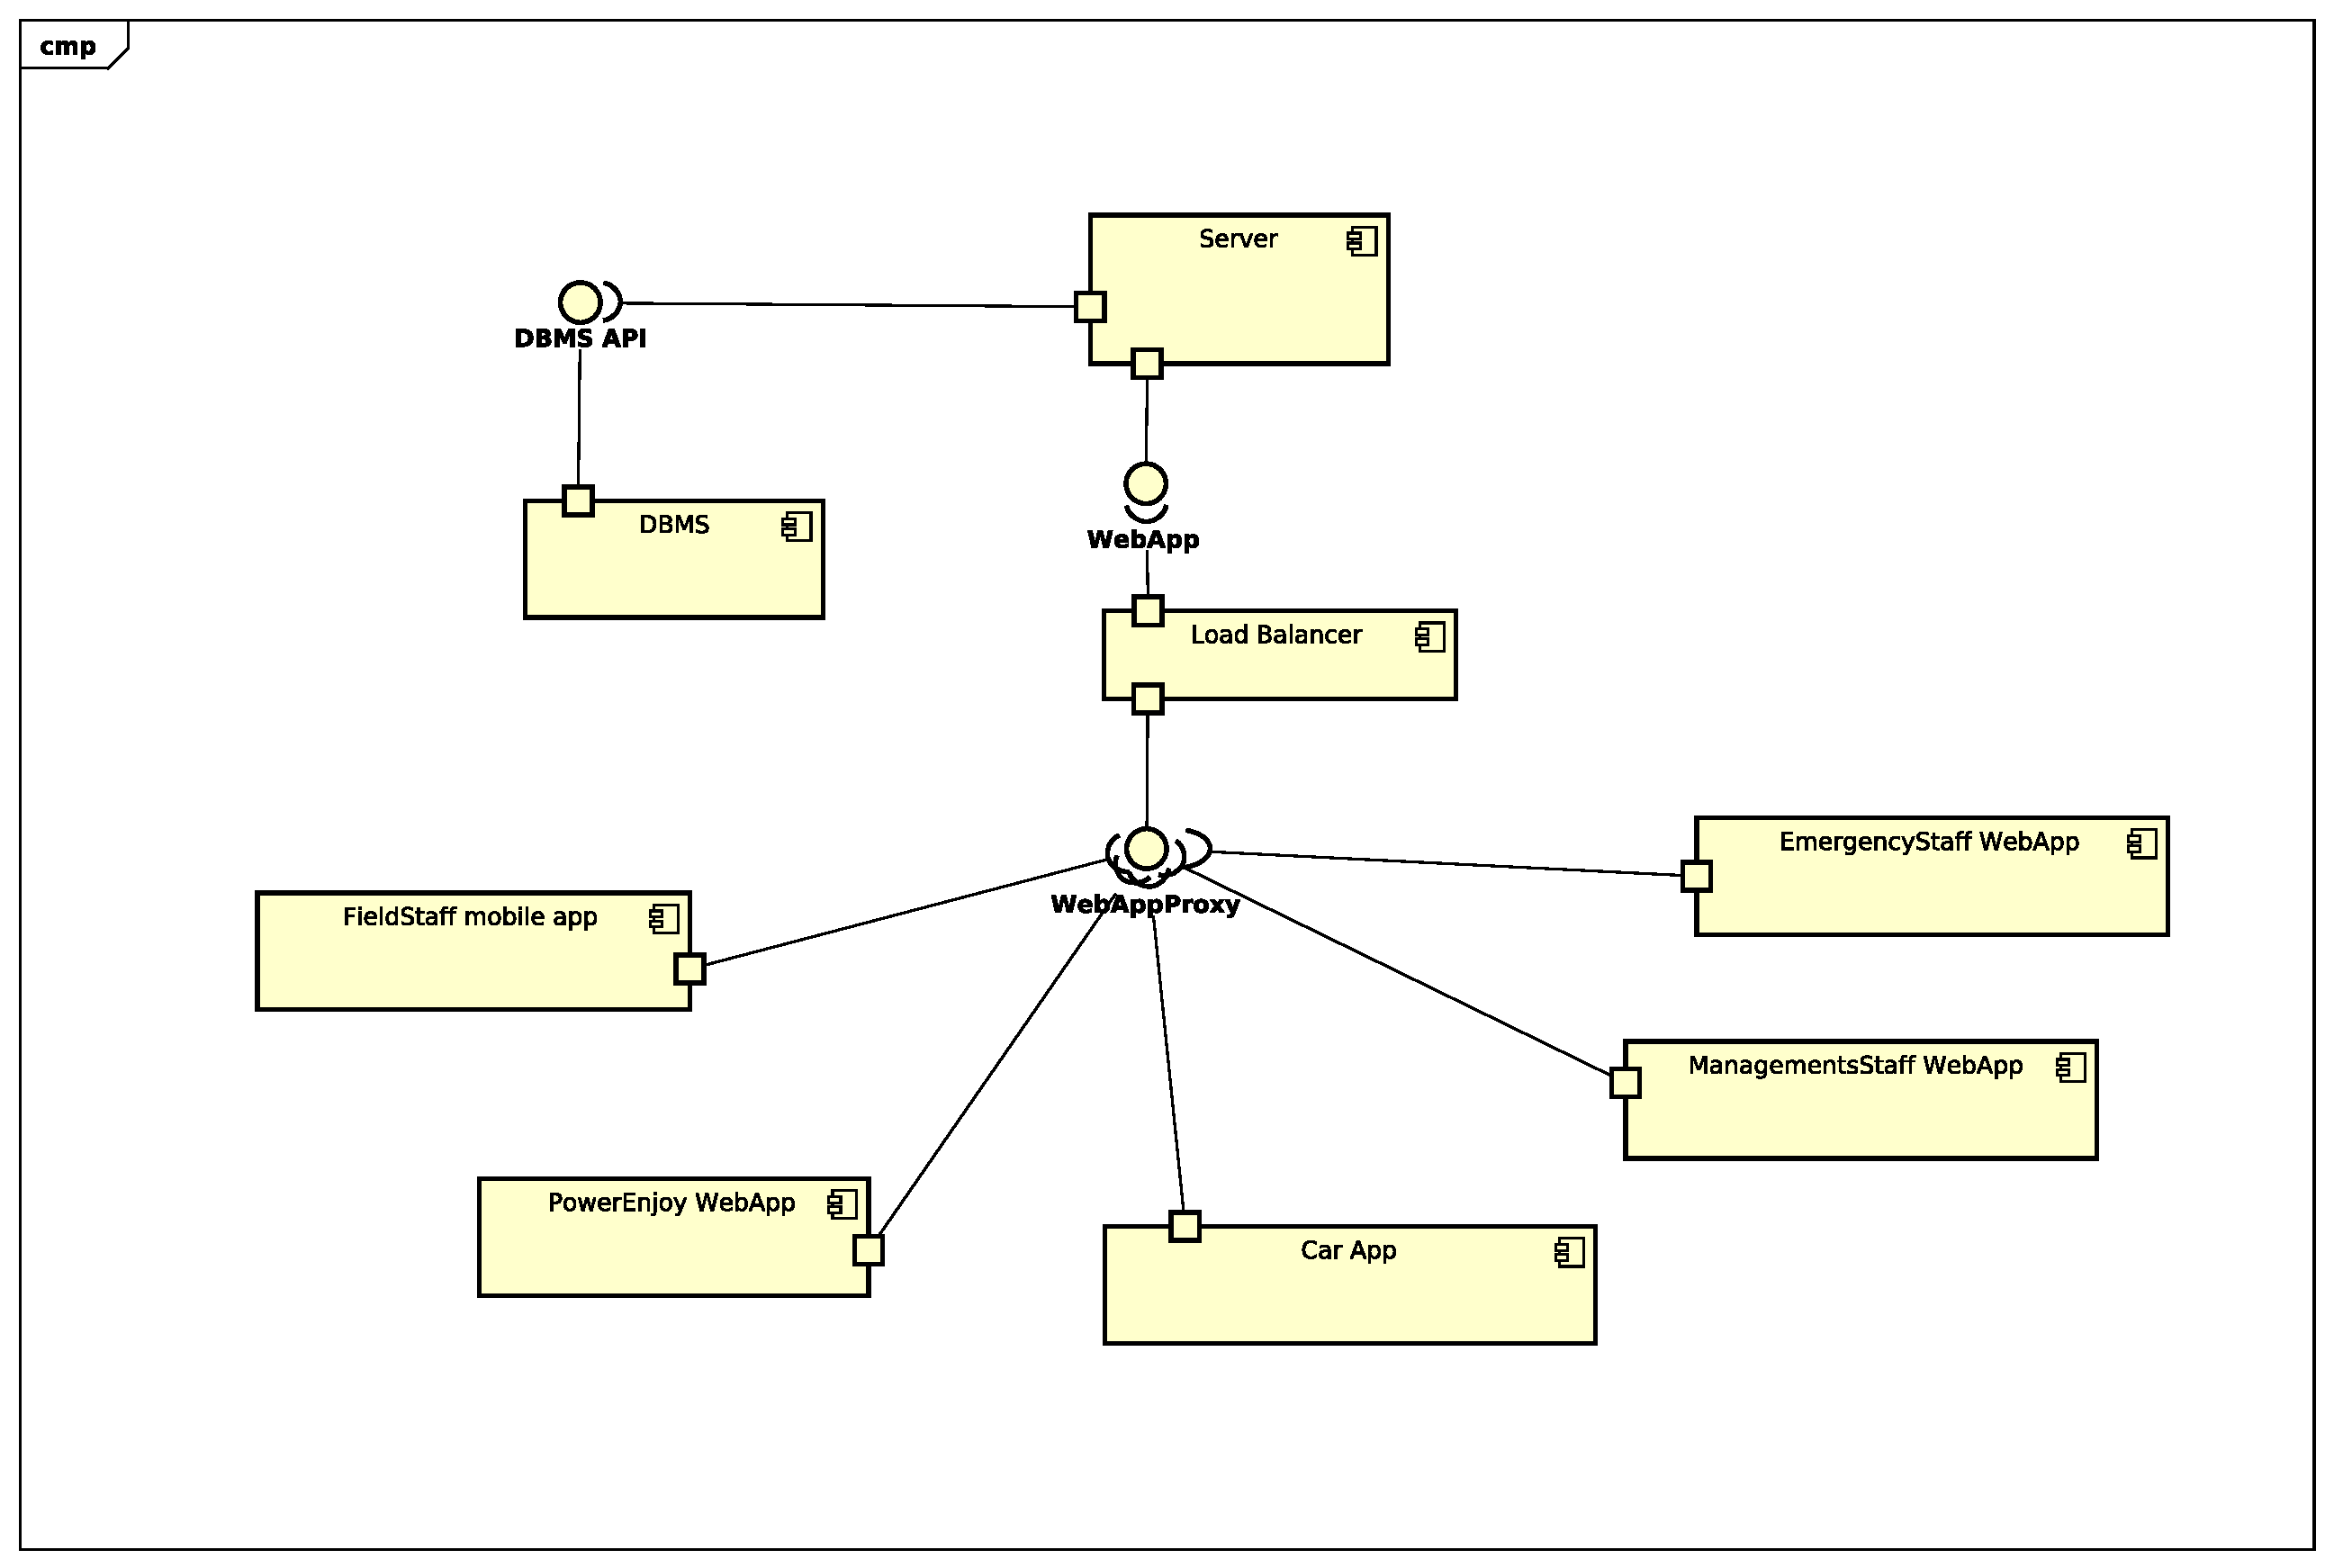
\includegraphics[scale=0.25]{./ComponentDiagrams/HighLevel.pdf}% "%" necessario
				\caption{High level architecture overview}
			\end{figure}
	\subsection{Component view}
		In this section the architectural overview is exploded into subcomponents, focusing on the server decomposition rather than the applications decomposition.\\
		A first global low-level component is presented to show the relations and the interfaces between all components, then the thematic areas of the diagram will be highlighted in separated sub diagrams, completed with textual comment of the individual components.
		\begin{landscape}
			\noindent
			\begin{figure}[H]
				\centering
				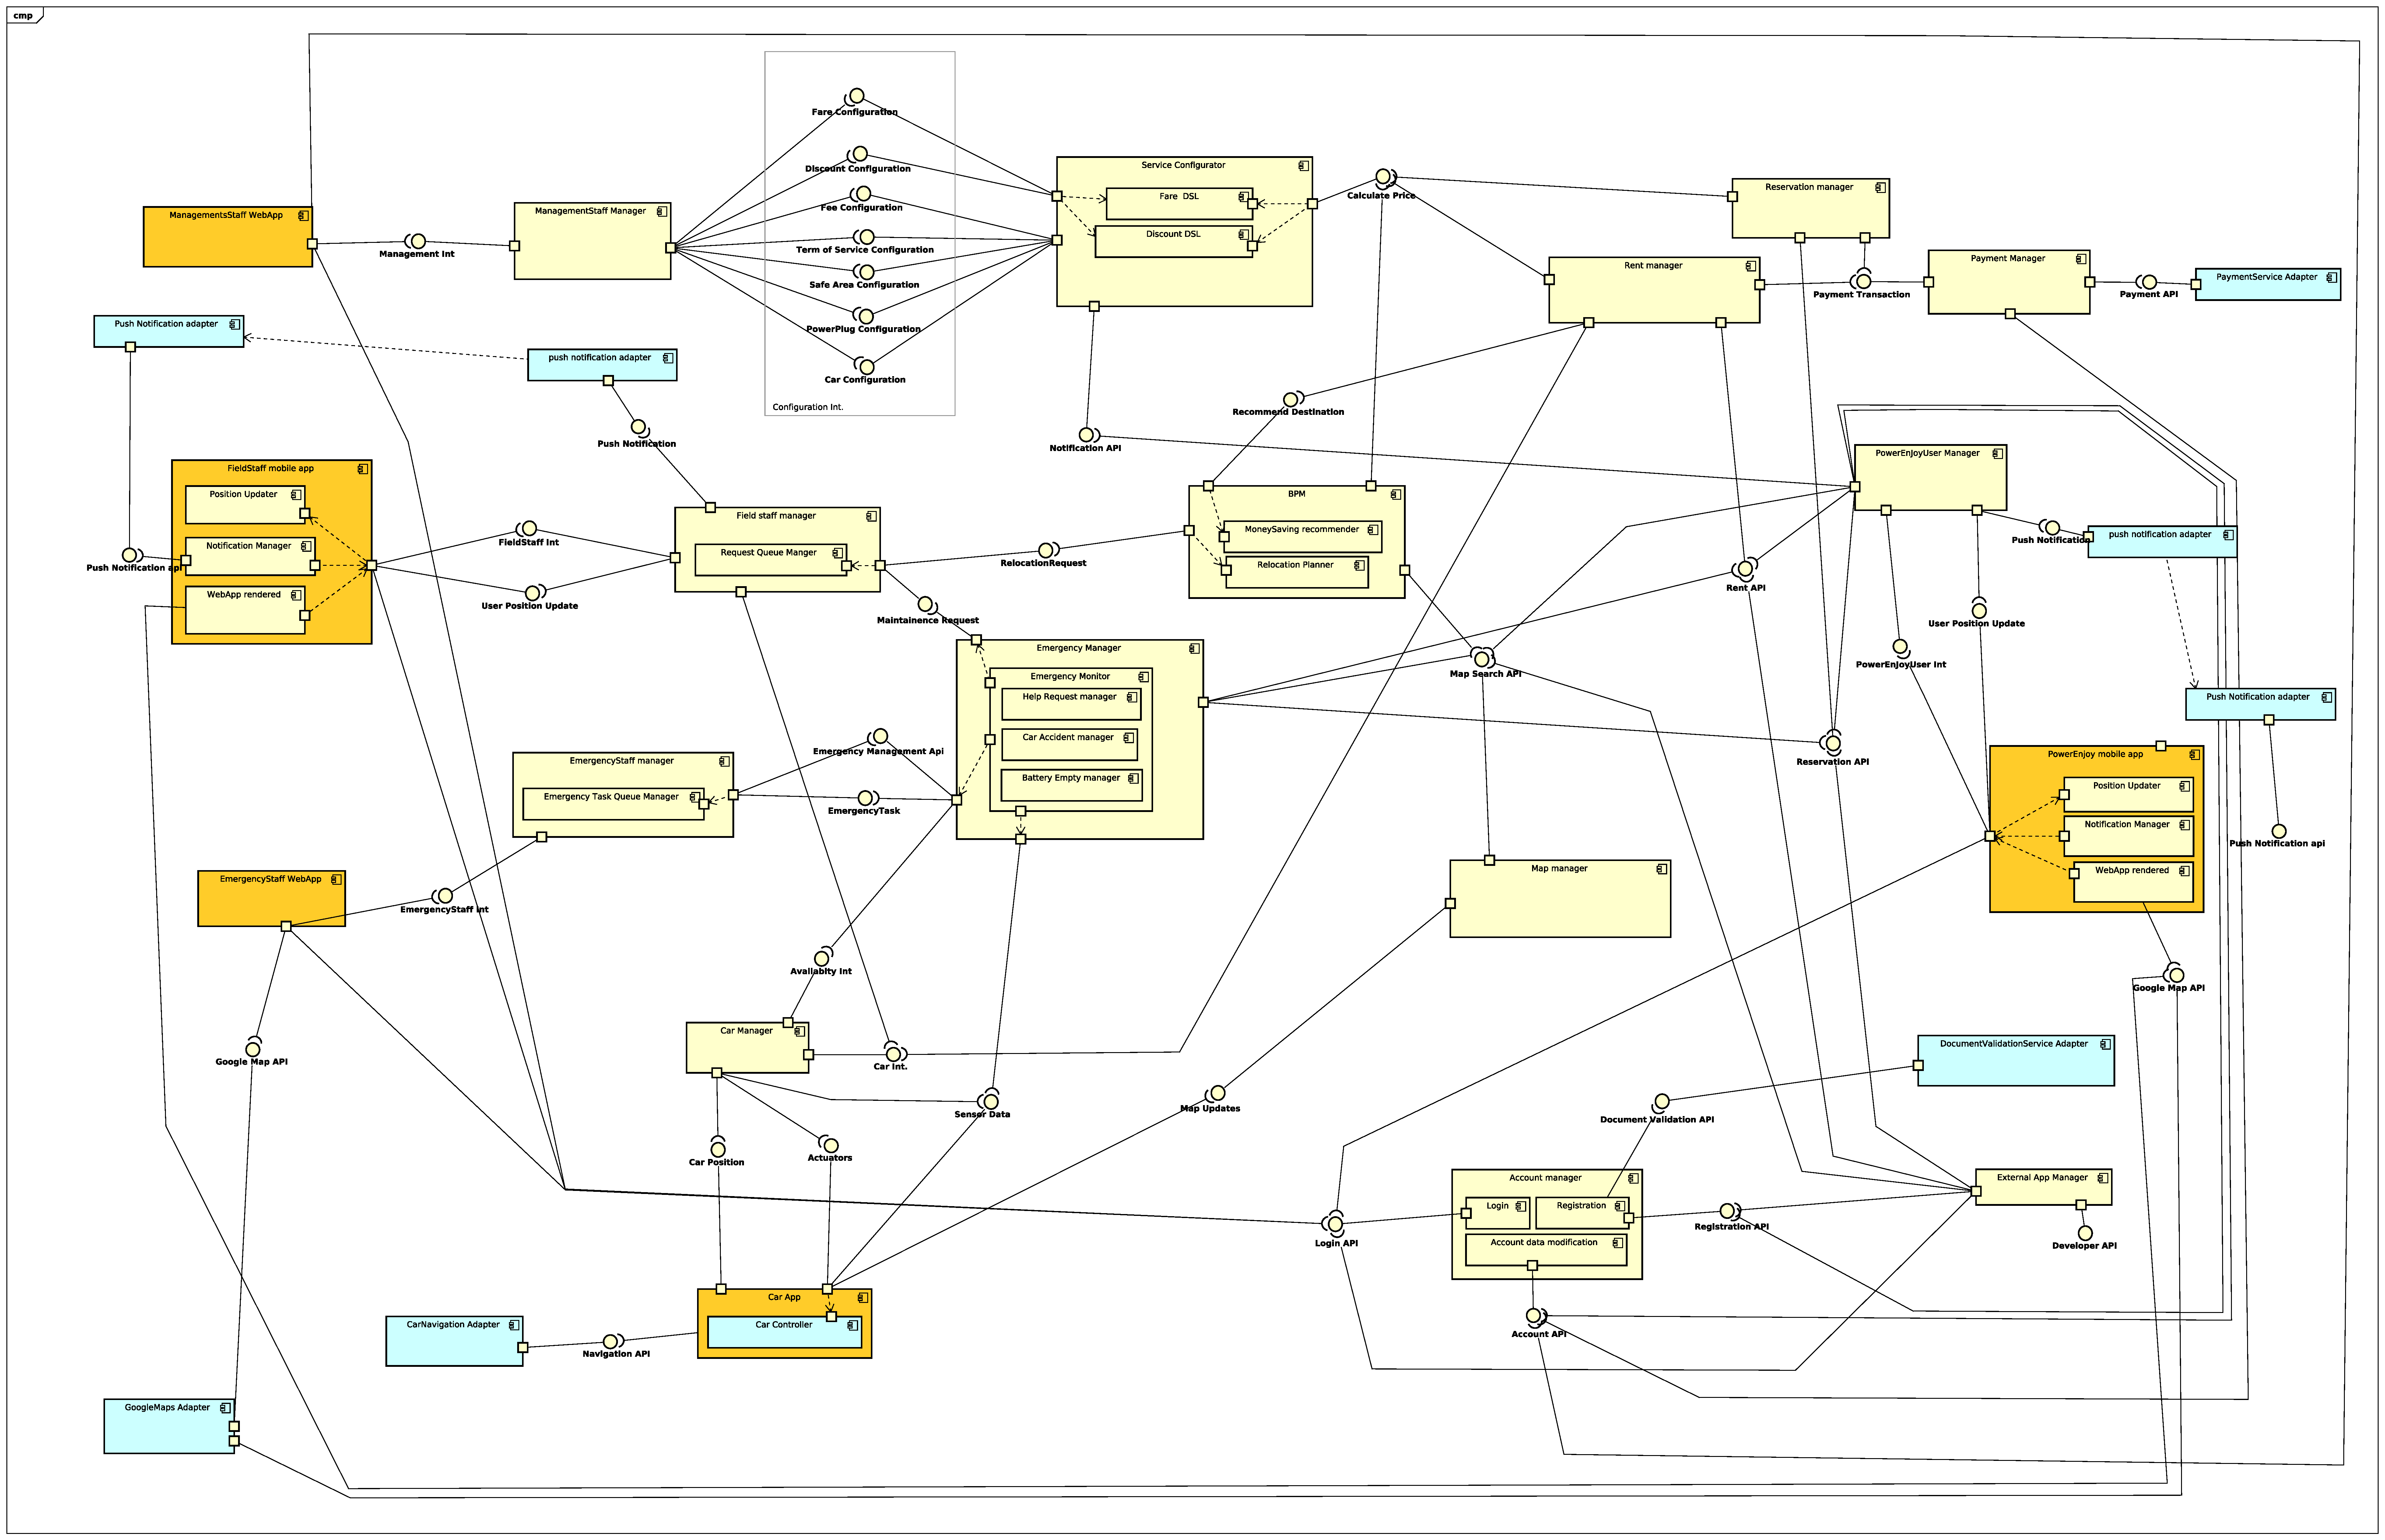
\includegraphics[scale=0.1068]{./ComponentDiagrams/LowLevel.pdf}% "%" necessario
				\caption{Low level architecture overview}
			\end{figure}
		\end{landscape}	
	\subsubsection*{Global considerations}
	\begin{itemize}
		\item{ Orange components correspond to the applications }
		\item{ Yellowish components are the decomposition of server }
		\item{ Blueish components correspond external service's adapters }
		\item{ The server components are modelled to be compliant with Java EE technology. In particular each component will exploit Java EE persistence framework to synchronize data with the DBMS (that is the reason no component has explicit use of DBMS API).  }
		\item{ Each application connect to a single proxy component on the server, that is created every time an application log-in as that user type.\\ Those components will be Java EE servlet, which can connect with other business beans.\\
		E.g: PowerEnJoyUser log-in from mobile app (connecting to <Account manager>'s Login API), then a <PowerEnJoy User Manager> is created and associated to the connection with the app session.   }
		\item{ <Rent manager> and <Reservation manager> are stateful entity beans and are created every time a corresponding rent / reservation is issued for creation.  }
		\item{ <Account manager>, <Payment manager>, <external app manager> and <service configurator> are stateless beans in order to increase scalability and are pooled to avoid creation overhead, since are stateless. }
		\item{ <Account manager>, <Payment manager>, <external app manager> and <service configurator> are stateless beans in order to increase scalability and are pooled to avoid creation overhead, since are stateless. }
		\item{ <BPM> component is scheduled to execute its cycle every 15 minutes. }
		\item{ <Map manager> offer services to all other components, so it keeps cached versions of the computed data to speed up further requests of same API call. }
		\item{  <Emergency manager> contains several event observers. Every time an event is registered (e.g: car malfunctioning), generate a task and assign to other component's queue (<Emergency/Field staff manger>). In addition this component act as API aggregator for the <Emergency staff manager>. }
	\end{itemize}

\clearpage
\subsubsection*{Car system}

	\subsubsection{Car app}
	Application running on the car screen, responsible of displaying current rent price, enabling money saving option, enable stopover mode, send car position and battery updates to server and control car actuators such as door's and power's lock. In addition polls the server for map updates (new safe areas / power plug slots) for the third party navigation system. 
		\subsubsection{Car controller}
		Car app subcomponent responsible of accessing car sensors and actuators through the car's ECU manufacturer APIs.
		\subsubsection{Car navigation adapter}
		Include navigation capabilities in the app exploiting third party software. Moreover is responsible of updating safe areas / power plug slots informations in the navigation system once an update is received.
	\subsubsection{Car manager}
	Component that receives position / battery charge updates from the associated car, and update the database accordingly. \\In addition offer rent manager and field staff manager an interface to control the car (lock/unlock, poweron/poweroff, ...)
	
	\begin{figure}[H]
		\centering
		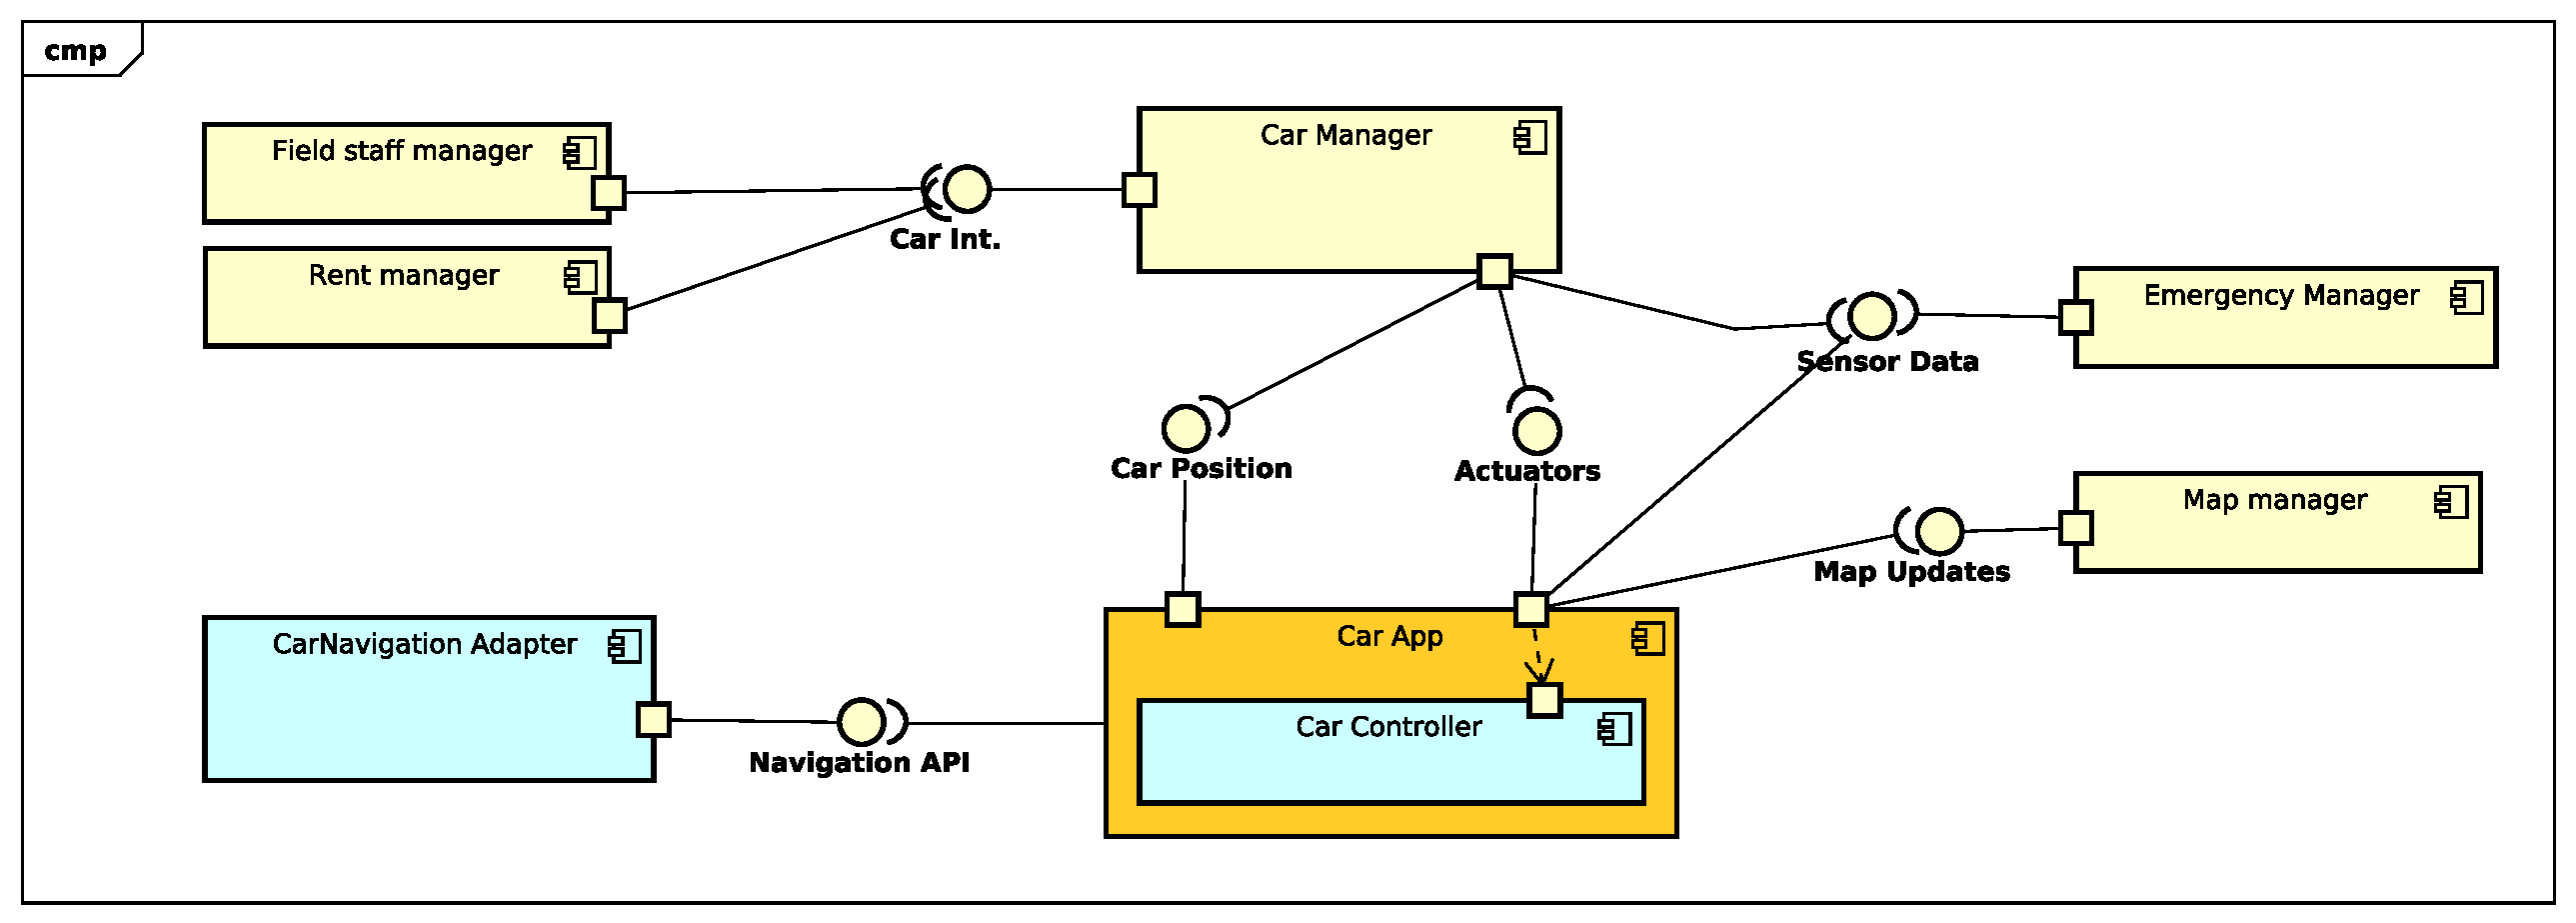
\includegraphics[scale=0.35]{./ComponentDiagrams/Car.pdf}% "%" necessario
		\caption{Car system related components}
	\end{figure}
	
\subsubsection*{PowerEnJoy app}
	
	\subsubsection{PowerEnJoyUser mobile app}
	Mobile app used by PowerEnJoy users to interact with the service. It gives the possibility to register as new user. After the initial login, enables the user to search for cars (near to its location or to an entered address) and reserve or rent an available car. Moreover permits to check the status of a reservation, unlock an available car once nearby and modify account informations. It displays push notifications for updated terms of services (including fares and discounts) .
		\subsubsection{Position updater}
		Periodically retrieve position informations and send to the server.
		\subsubsection{Notification manager}
		Listen for push notification from the server about updated terms of services (including fares and discounts) and display on the smart device.
		\subsubsection{WebApp rendered}
		The app for smart device includes a renderer (web view) that runs the actual application (a webapp), in order to achieve the maximum code portability without sacrifice native look in notifications nor loosing the marketing possibilities of smart device's online app markets.
	\subsubsection{PowerEnJoyUser manager}
	Dual component of PowerEnJoyUser mobile app on the server, it is created after the internal webapp logins, and it's associated to the webapp session. Provide an unified access to all the interfaces for performing rents and reservations. Updates the user's location on database. Notify the app through push notification once term of services are updated.
	\subsubsection{GoogleMaps adapter}
	Exploit Google Maps services to convert addresses into coordinates and to display cars, power plug slots and the shortest path to reach them over an interactive map.
	\subsubsection{Push notification adapter}
	Exploits third party API (Google cloud messanging API) to send/receive push notifications to user's app.
	\subsubsection{Account manager}
	Handles login requests from all the applications. Register new users, validating  submitted documents. Permit users to modify account informations. Provide PIN / password recovery capabilities.
		\subsubsection{Registration }
		For each registration request it completes the validation steps, generates password and PIN codes and sends a confirmation email with user's credentials.
		\subsubsection{Login}
		Handle a single login request. Create an appropriate dual component on server for the app that request the login (based on the user account type).
		\subsubsection{Account data modification }
		Update users information on database.
	\subsubsection{DocumentValidationService adapter}
	Exploit external service to validate documents.
	
	\subsubsection{Map manager}
	\subsubsection{Reservation manager}
	\subsubsection{Rent manager}
	
	\subsubsection{Payment manager}
	\subsubsection{PaymentService adapter}
	
	\subsubsection{BPM}
		\subsubsection{MoneySaving recommender }
	
	\subsubsection{External app manager}
	
	\begin{figure}[H]
		\centering
		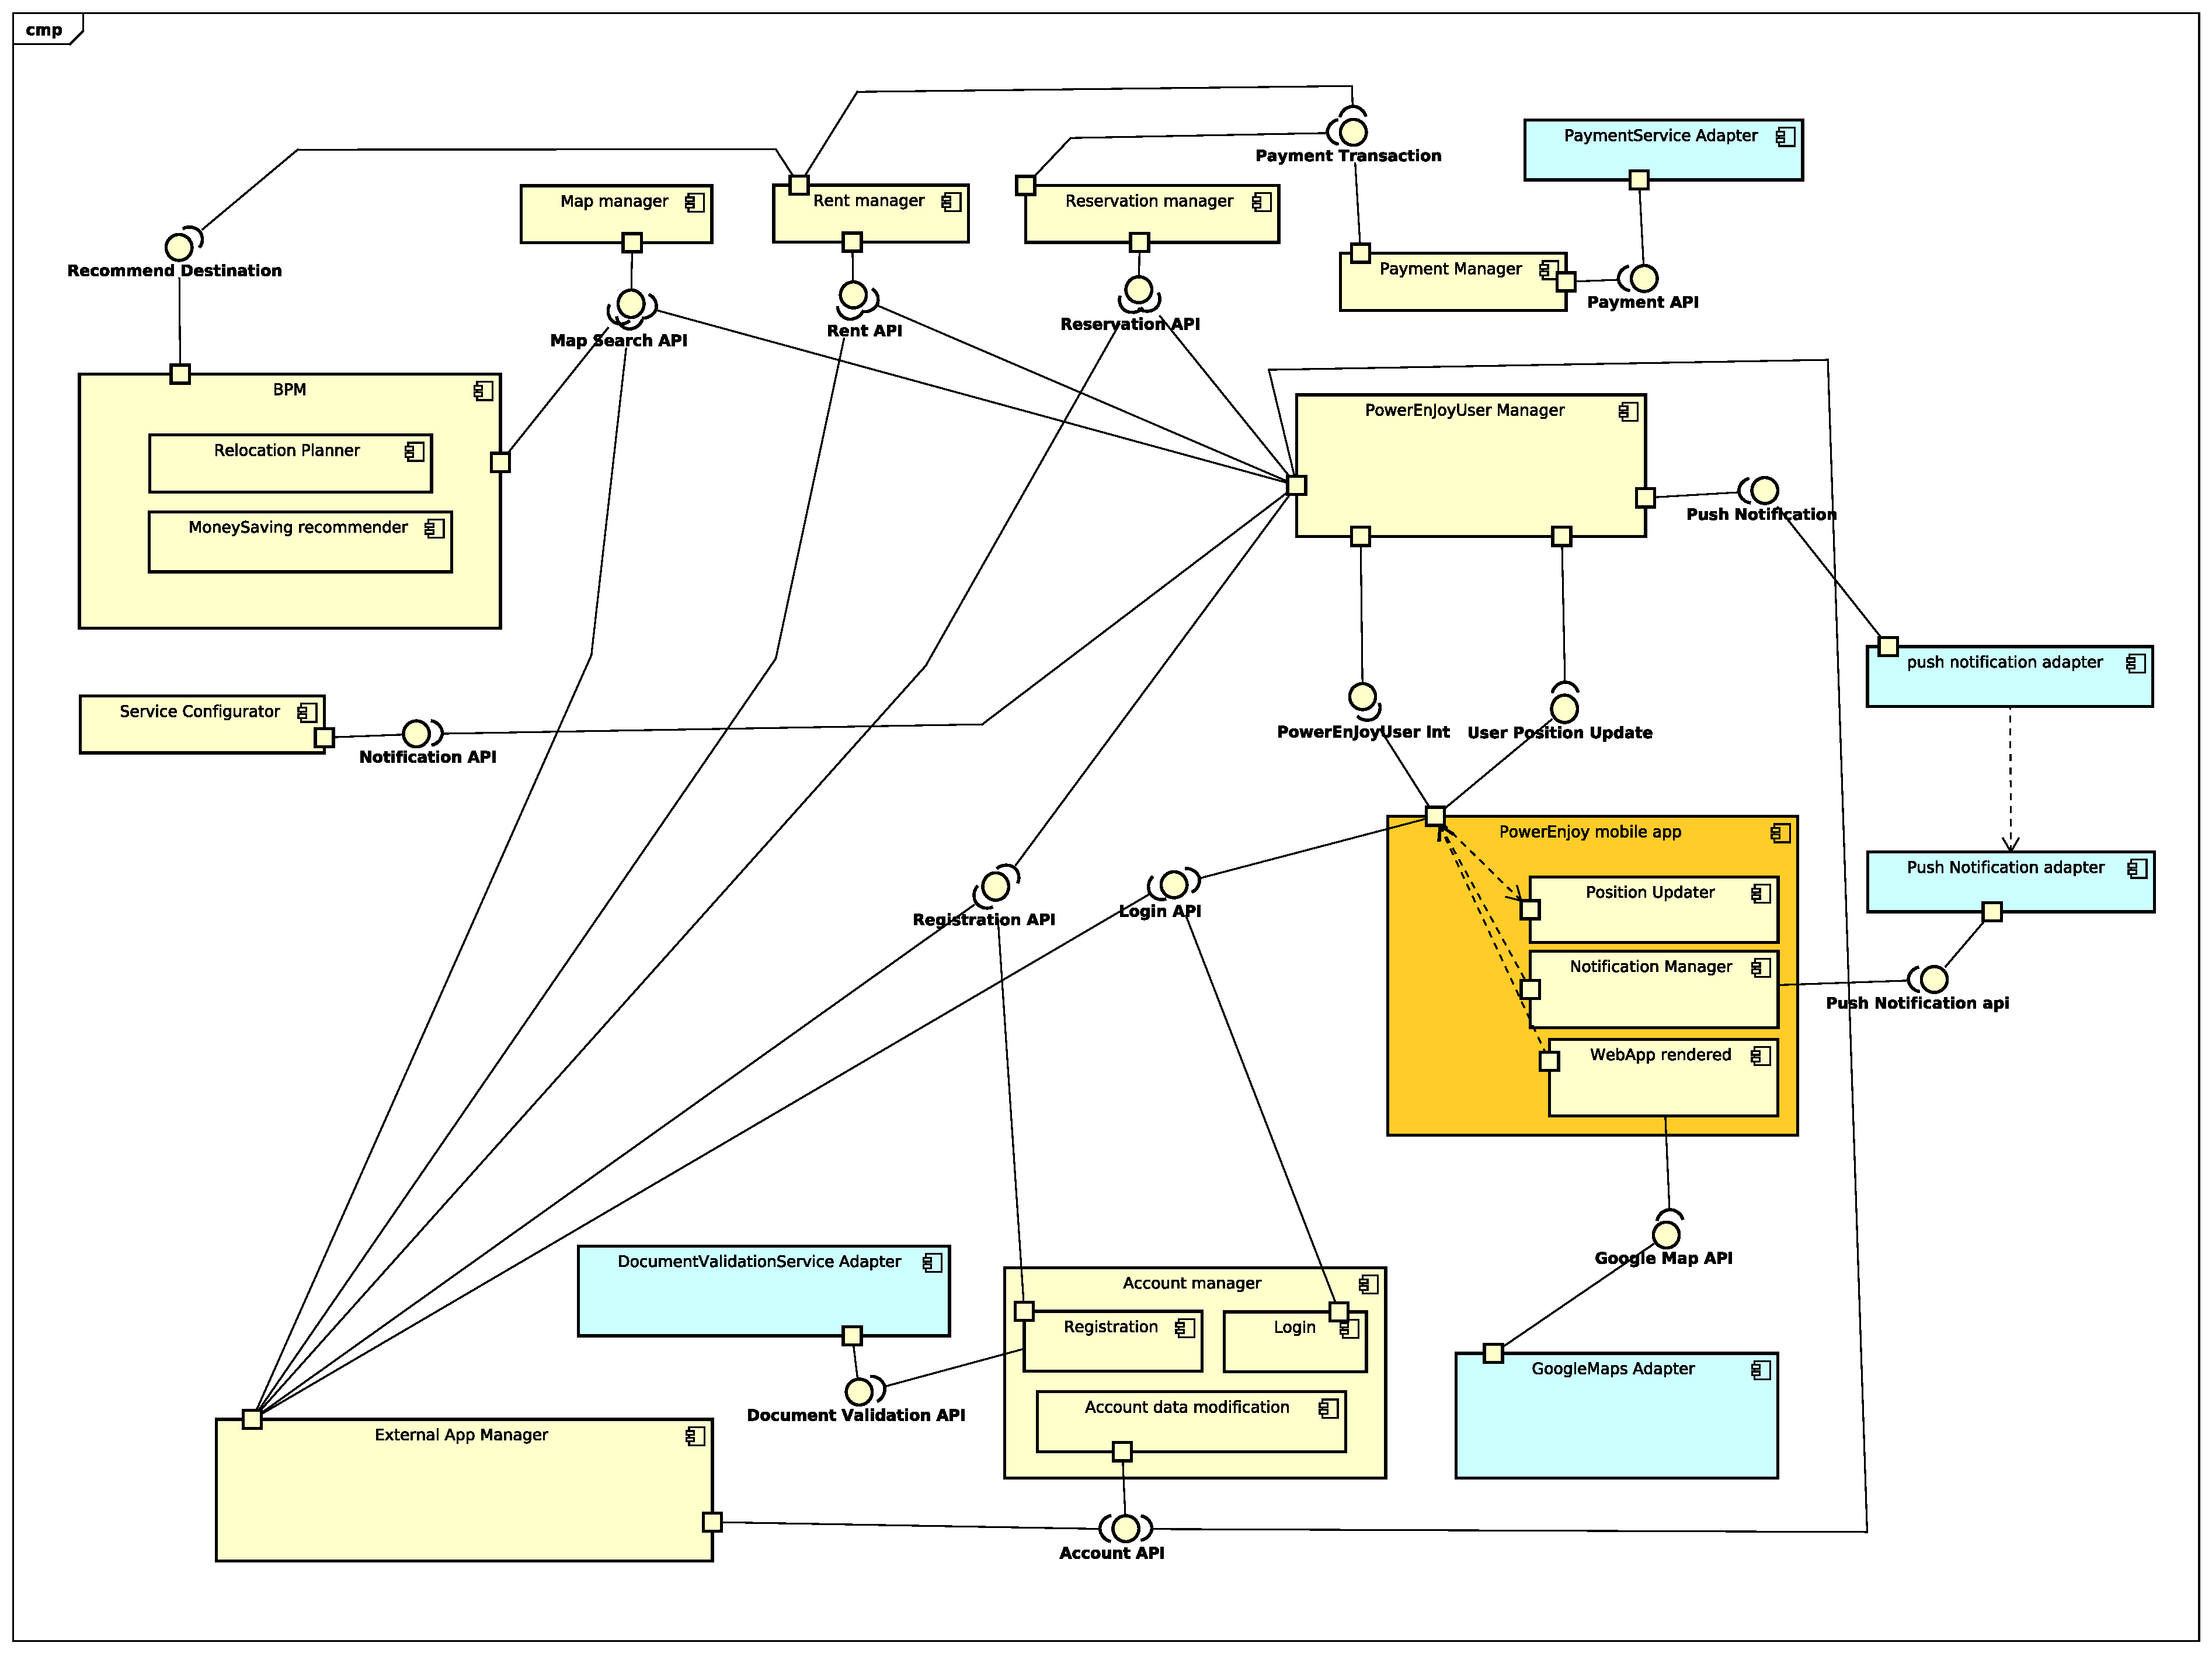
\includegraphics[scale=0.24]{./ComponentDiagrams/PowerEnjoyuser.pdf}% "%" necessario
		\caption{PowerEnJoy app related components}
	\end{figure}
	
	
\subsubsection*{Field staff app}
	
	\subsubsection{Field staff mobile app}
	Mobile app used by field staff users to receive notification of relocation/maintenance requests. After the initial login, enables the user to view list of assigned requests, and for each one of them shows information (including the location) about the target car. Through this app is also possible to unlock and power-on assigned cars, as well as contact emergency staff for support.
		\subsubsection{Position updater}
		Periodically retrieve position informations and send to the server.
		\subsubsection{Notification manager}
		Listen for push notification from the server about new tasks and display on the smart device.
		\subsubsection{WebApp rendered}
		The app for smart device includes a renderer (web view) that runs the actual application (a webapp), in order to achieve the maximum code portability without sacrifice native look in notifications nor loosing the marketing possibilities of smart device's online app markets.
	\subsubsection{Field staff manager}
	Dual component of Field staff mobile app on the server, it is created after the internal webapp logins, and it's associated to the webapp session. Provide and manage a queue of all assigned requests and sends push notifications to the app once a new request is registered. It also updates the field staff user's location on database.
		\subsubsection{Request Queue manager}
		Manage the emergency request queue of a field staff user, it provides an interface to be assigned tasks to BPM and Emergency manager.
	\subsubsection{Push notification adapter}
	Exploits third party API (Google cloud messanging API) to send/receive push notifications of new requests to the field staff user's app.
	\subsubsection{Relocation planner }
	BPM subcomponent that computes relocations in order to remove charged cars from power plug slots, bring empty battery cars to power plug slots and fairly distribute cars over territory. Computed relocations are assigned to field staff users.
	\begin{figure}[H]
		\centering
		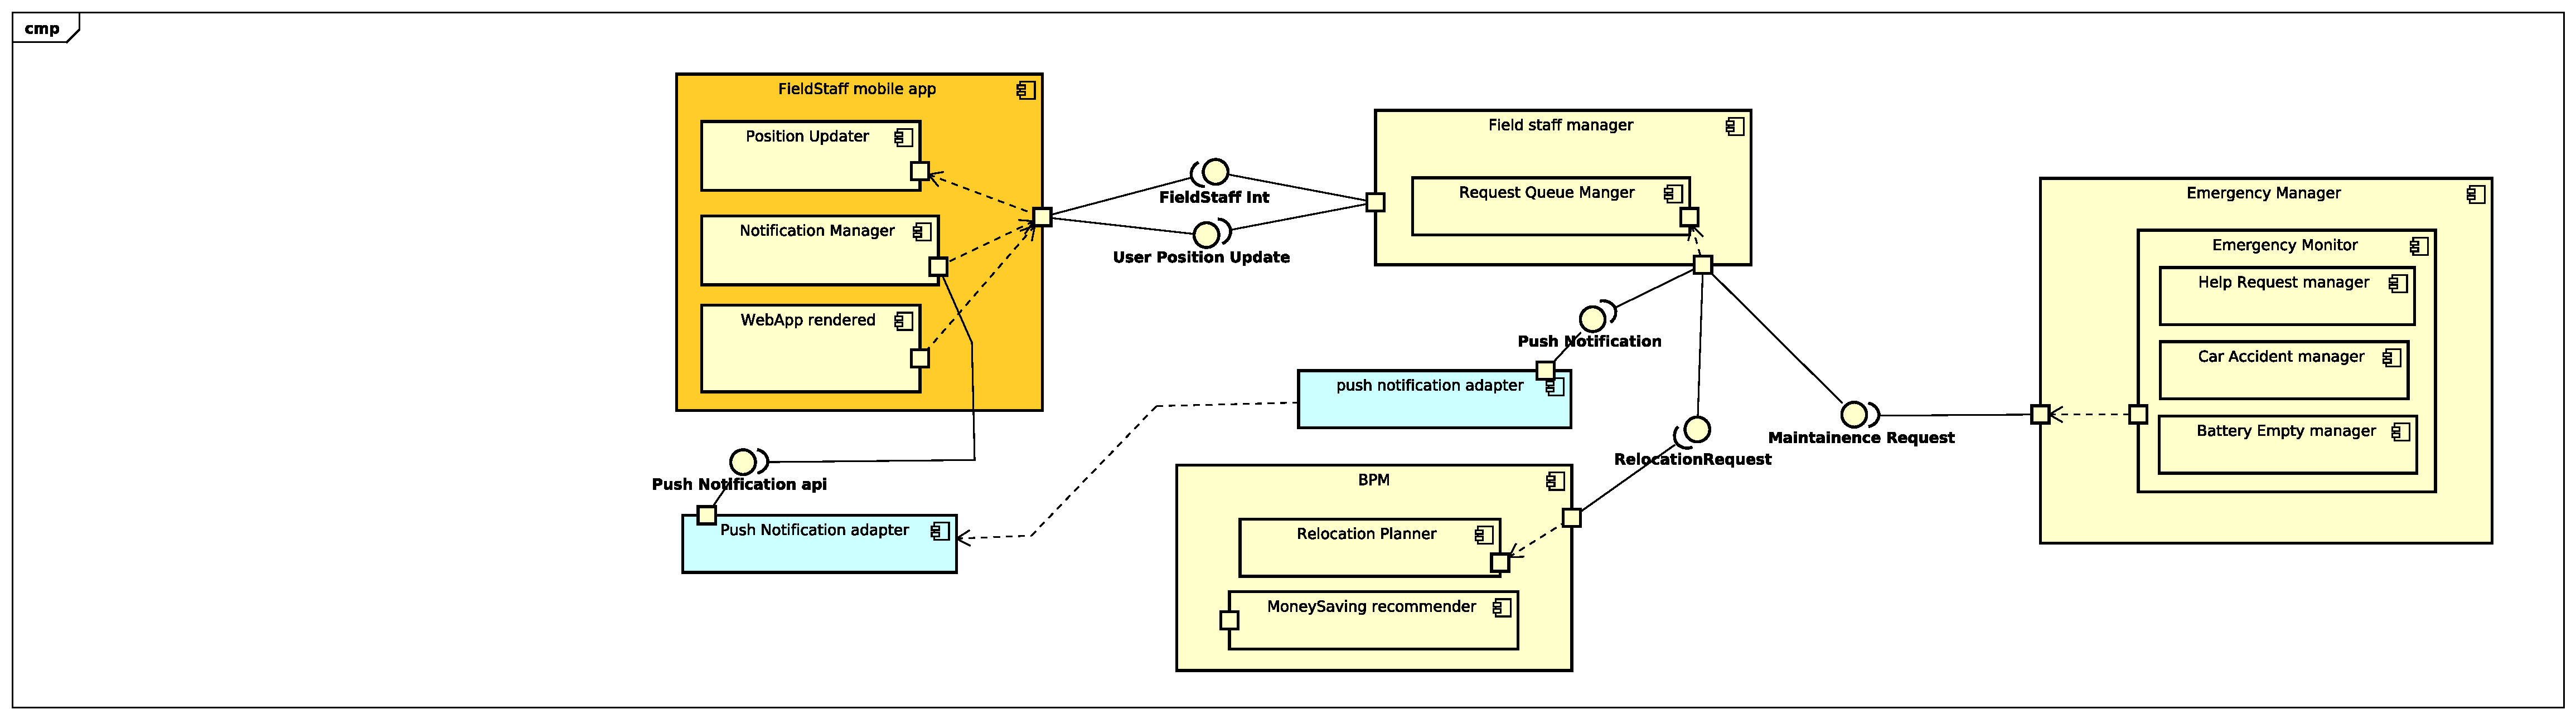
\includegraphics[scale=0.21]{./ComponentDiagrams/FieldStaff.pdf}% "%" necessario
		\caption{Field staff app related components}
	\end{figure}
	
	
\subsubsection*{Emergency staff webapp}

	\subsubsection{Emergency staff webapp}
	Webapp (runs inside browser) used by emergency staff users to receive notification of and handle emergency situations. After the initial login, enables the user to view list of assigned emergency tasks, and for each one of them displays on a map an overview of the emergency containing all related informations.
	\subsubsection{Emergency staff manager}
	Dual component of Emergency staff webapp on the server, it is created after the webapp logins, and it's associated to the webapp session. Provide and manage a queue of all assigned tasks. In addition it interfaces with Emergency manager to cancel rents/reservations, get an overview of the map and assign requests to field staff users.
		\subsubsection{Request Queue manager}
		Manage the emergency task queue of an emergency staff user, it provides an interface to be assigned tasks.
	\subsubsection{Emergency manager}
	This component detect car's and user's emergencies, and assign them as task to the field staff users (maintenance requests) or  emergency staff users (emergency task). Moreover aggregate some interfaces from Rent/Reservation/Field staff managers in order to empower the emergency staff in resolving their tasks. It automatically handles simpler task, such as set cars as broken (thus unavailable) after a car accident is registered or assign a maintenance request after a car malfunctioning is registered. \par See low level component view for complete overview of interactions with other components.
		\subsubsection{Emergency monitor}
		Contains several subcomponents specialized in recognizing a single type of emergency, and provide them the data needed. Collect usage data from car's sensors in order to detect malfunctioning and interprets the absence of car response as an accident after a timeout.  
	\begin{figure}[H]
		\centering
		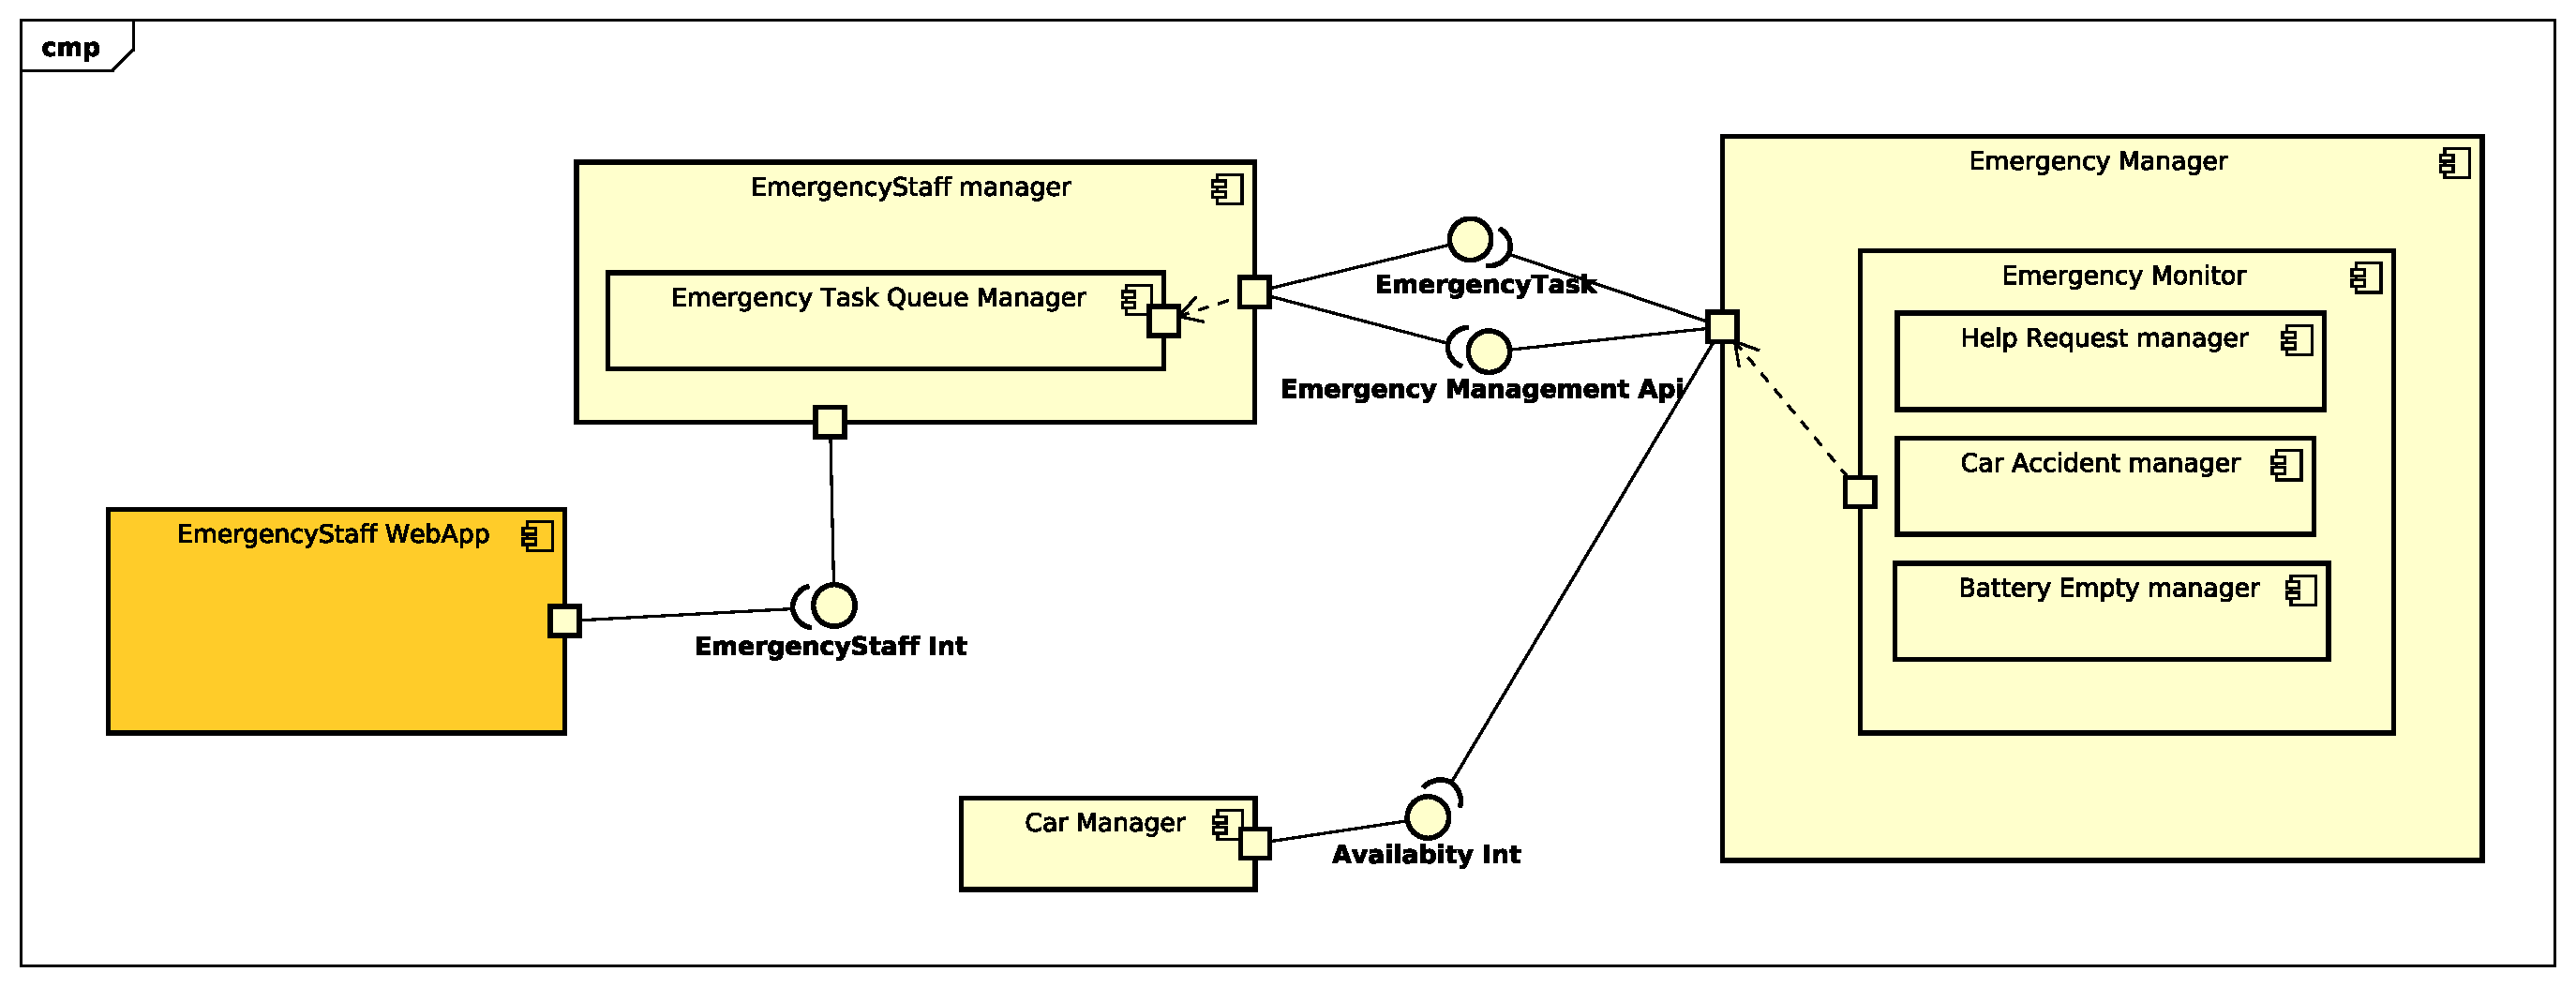
\includegraphics[scale=0.35]{./ComponentDiagrams/EmergencyStaff.pdf}% "%" necessario
		\caption{Emergency staff app related components}
	\end{figure}
	
	
\subsubsection*{Management staff webapp}

	\subsubsection{Management staff webapp}
	Webapp (runs inside browser) used by management staff users to configure all service's parameter. After the initial login, enables the user to configure fares, discounts, fees, term of services and add/remove safe areas/power plug slots/cars.
	\subsubsection{Management staff manager}
	Dual component of the Management staff webapp on the server, it is created after the webapp logins, and it's associated to the webapp session. Redirects all users request for configuration operation to the Service Configurator.
	\subsubsection{Service Configurator}
	Component that provides an interface to modify every parameter of service. It is polled by PowerEnJoyUser manager to find out whether fares/fee/discounts/term of services have been updated. Moreover it is called by BPM/Rent manager/Reservation manager to compute prices and fees, since for flexibility reasons those informations are saved as DSL scripts (see Fare DSL, Discount DSL).
		\subsubsection{Fare DSL}
		Interpreter of a specific DSL (Domain Specific Language) to configure and compute fares. It stores each fare as a script,  dynamically interpreted when a price should be calculated. The DSL is specifically designed to mimic Microsoft EXCEL formulae syntax (extended with specific functions to access service parameters) in order to guarantee the faster learning curve to most part of the company's management personnel.\\
		E.g: 
		\begin{itemize}
			\item { = Rent.MOVING\_TIME() * 0.50 + Rent.STOP\_TIME() * 0.15     \\time based fare, considering stopover (0.50\euro/minute for rent, 0.15\euro/minute for stopover)}
			\item { = IF( Rent.KM() > 10; (Rent.KM()-10) * 0.05; 0) 			      \\ km based fare, start after a minimum of 10 km 0.05\euro/km}
		\end{itemize}
		\subsubsection{Discount DSL}
		Interpreter of a specific DSL (Domain Specific Language) to configure and compute discounts. It stores each discount as a script,  dynamically interpreted when a price should be calculated. The DSL is specifically designed to mimic Microsoft EXCEL formulae syntax (extended with specific functions to access service parameters) in order to guarantee the faster learning curve to most part of the company's management personnel.
		E.g: 
		\begin{itemize}
			\item { = IF( Rent.PASSENGERS()>2; -0.20 ; 0)     \\passenger discount of 20\%, if 2+ passengers (the returned value is multiplied by price and added to price as modifier, for an overcharge the returned value should be positive) }
		\end{itemize}
	\begin{figure}[H]
		\centering
		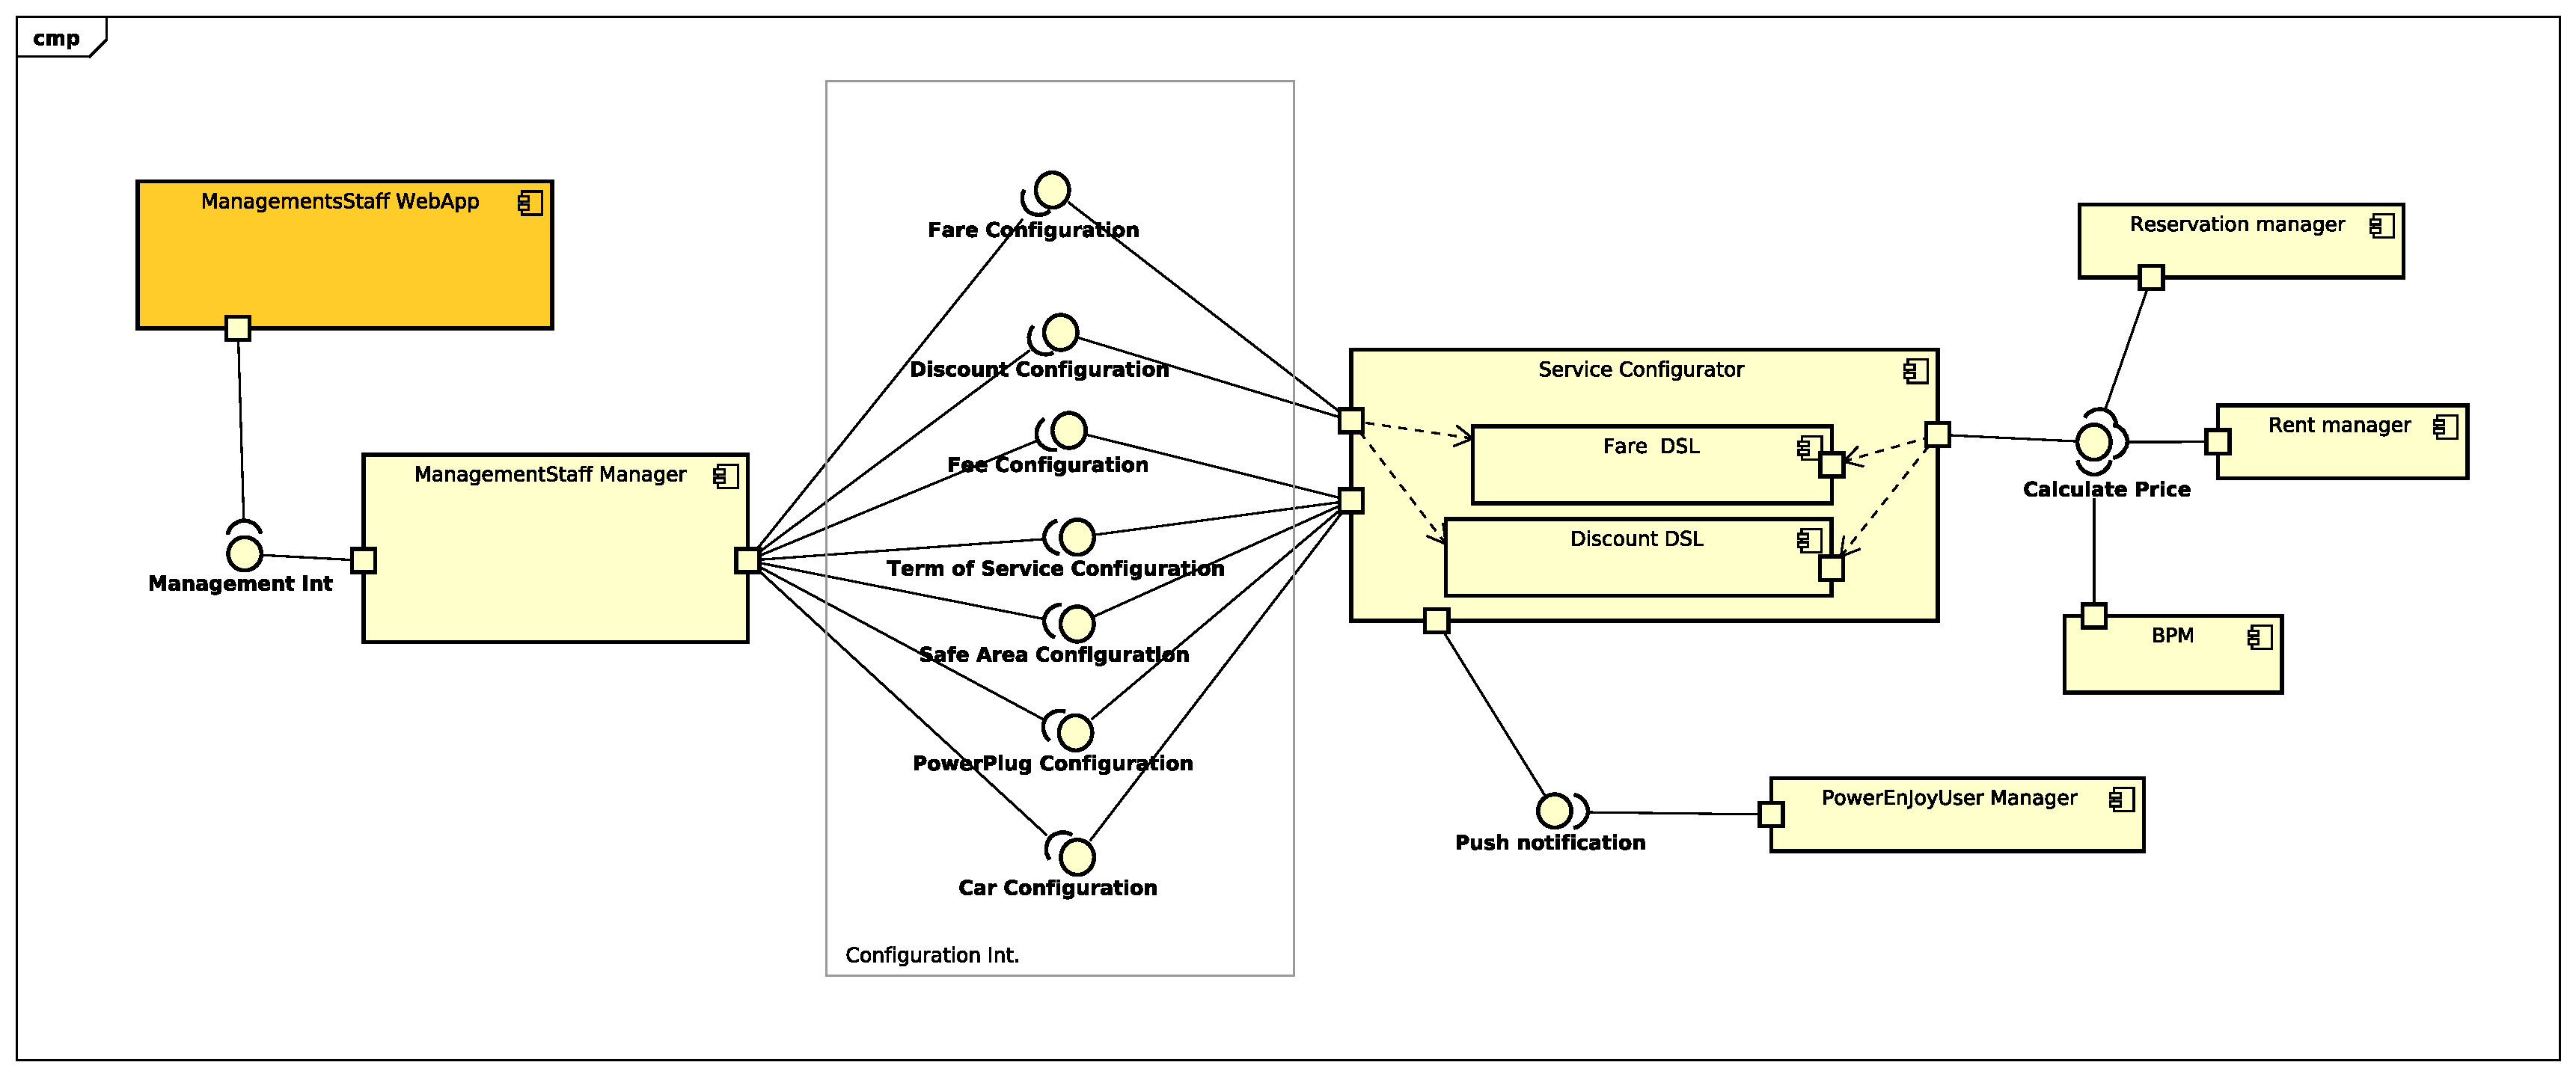
\includegraphics[scale=0.26]{./ComponentDiagrams/ManagementStaff.pdf}% "%" necessario
		\caption{Management staff app related components}
	\end{figure}
	
	
	\subsection{Deployment view}
	In the following figure we can see the deployment diagram. Here we show how the different components introduced in the Component View chapter are distributed into system's hardware components.
We have structured our diagram focusing on the workload of each component. We offer a real time service and we have to deal with these two principal data channels:
	\begin{itemize}
		\item All cars are connected send continuously data in order to be monitored. 
		\item Every client connected to the service via Web App should receive responses in real time.
	\end {itemize}
In order to fulfill these two needs we have introduced load balancers that distribute the load among servers. 
We have both N Web Servers and Business servers. The first type of server guarantees the fair management of clients requests and responses. The second type guarantees the fair management of services running on the Business Server.
We store Data in a database which is separated from the server. The Database is duplicated in a backup database.\\\\
This architecture is compliant with the Java EE model, which usually consist in 4 tier: 
		\begin{itemize}
			\item{ client presentation tier (user app, staff apps and car system)}
			\item{ web tier (Account, Car, PowerEnJoyUser and  ``* staff'' managers servlets)}
			\item{ business tier (Rent,Reservation,Payment,Emergency and Map managers;BPM)}
			\item{ data tier (DBMS; Backupper) }
		\end{itemize}
		This four tier architecture also increase the security of business data, through a second firewall before Business server, and the secrecy/security of strategic component's code such as BPM.
		
			\begin{figure}[H]
				\centering
				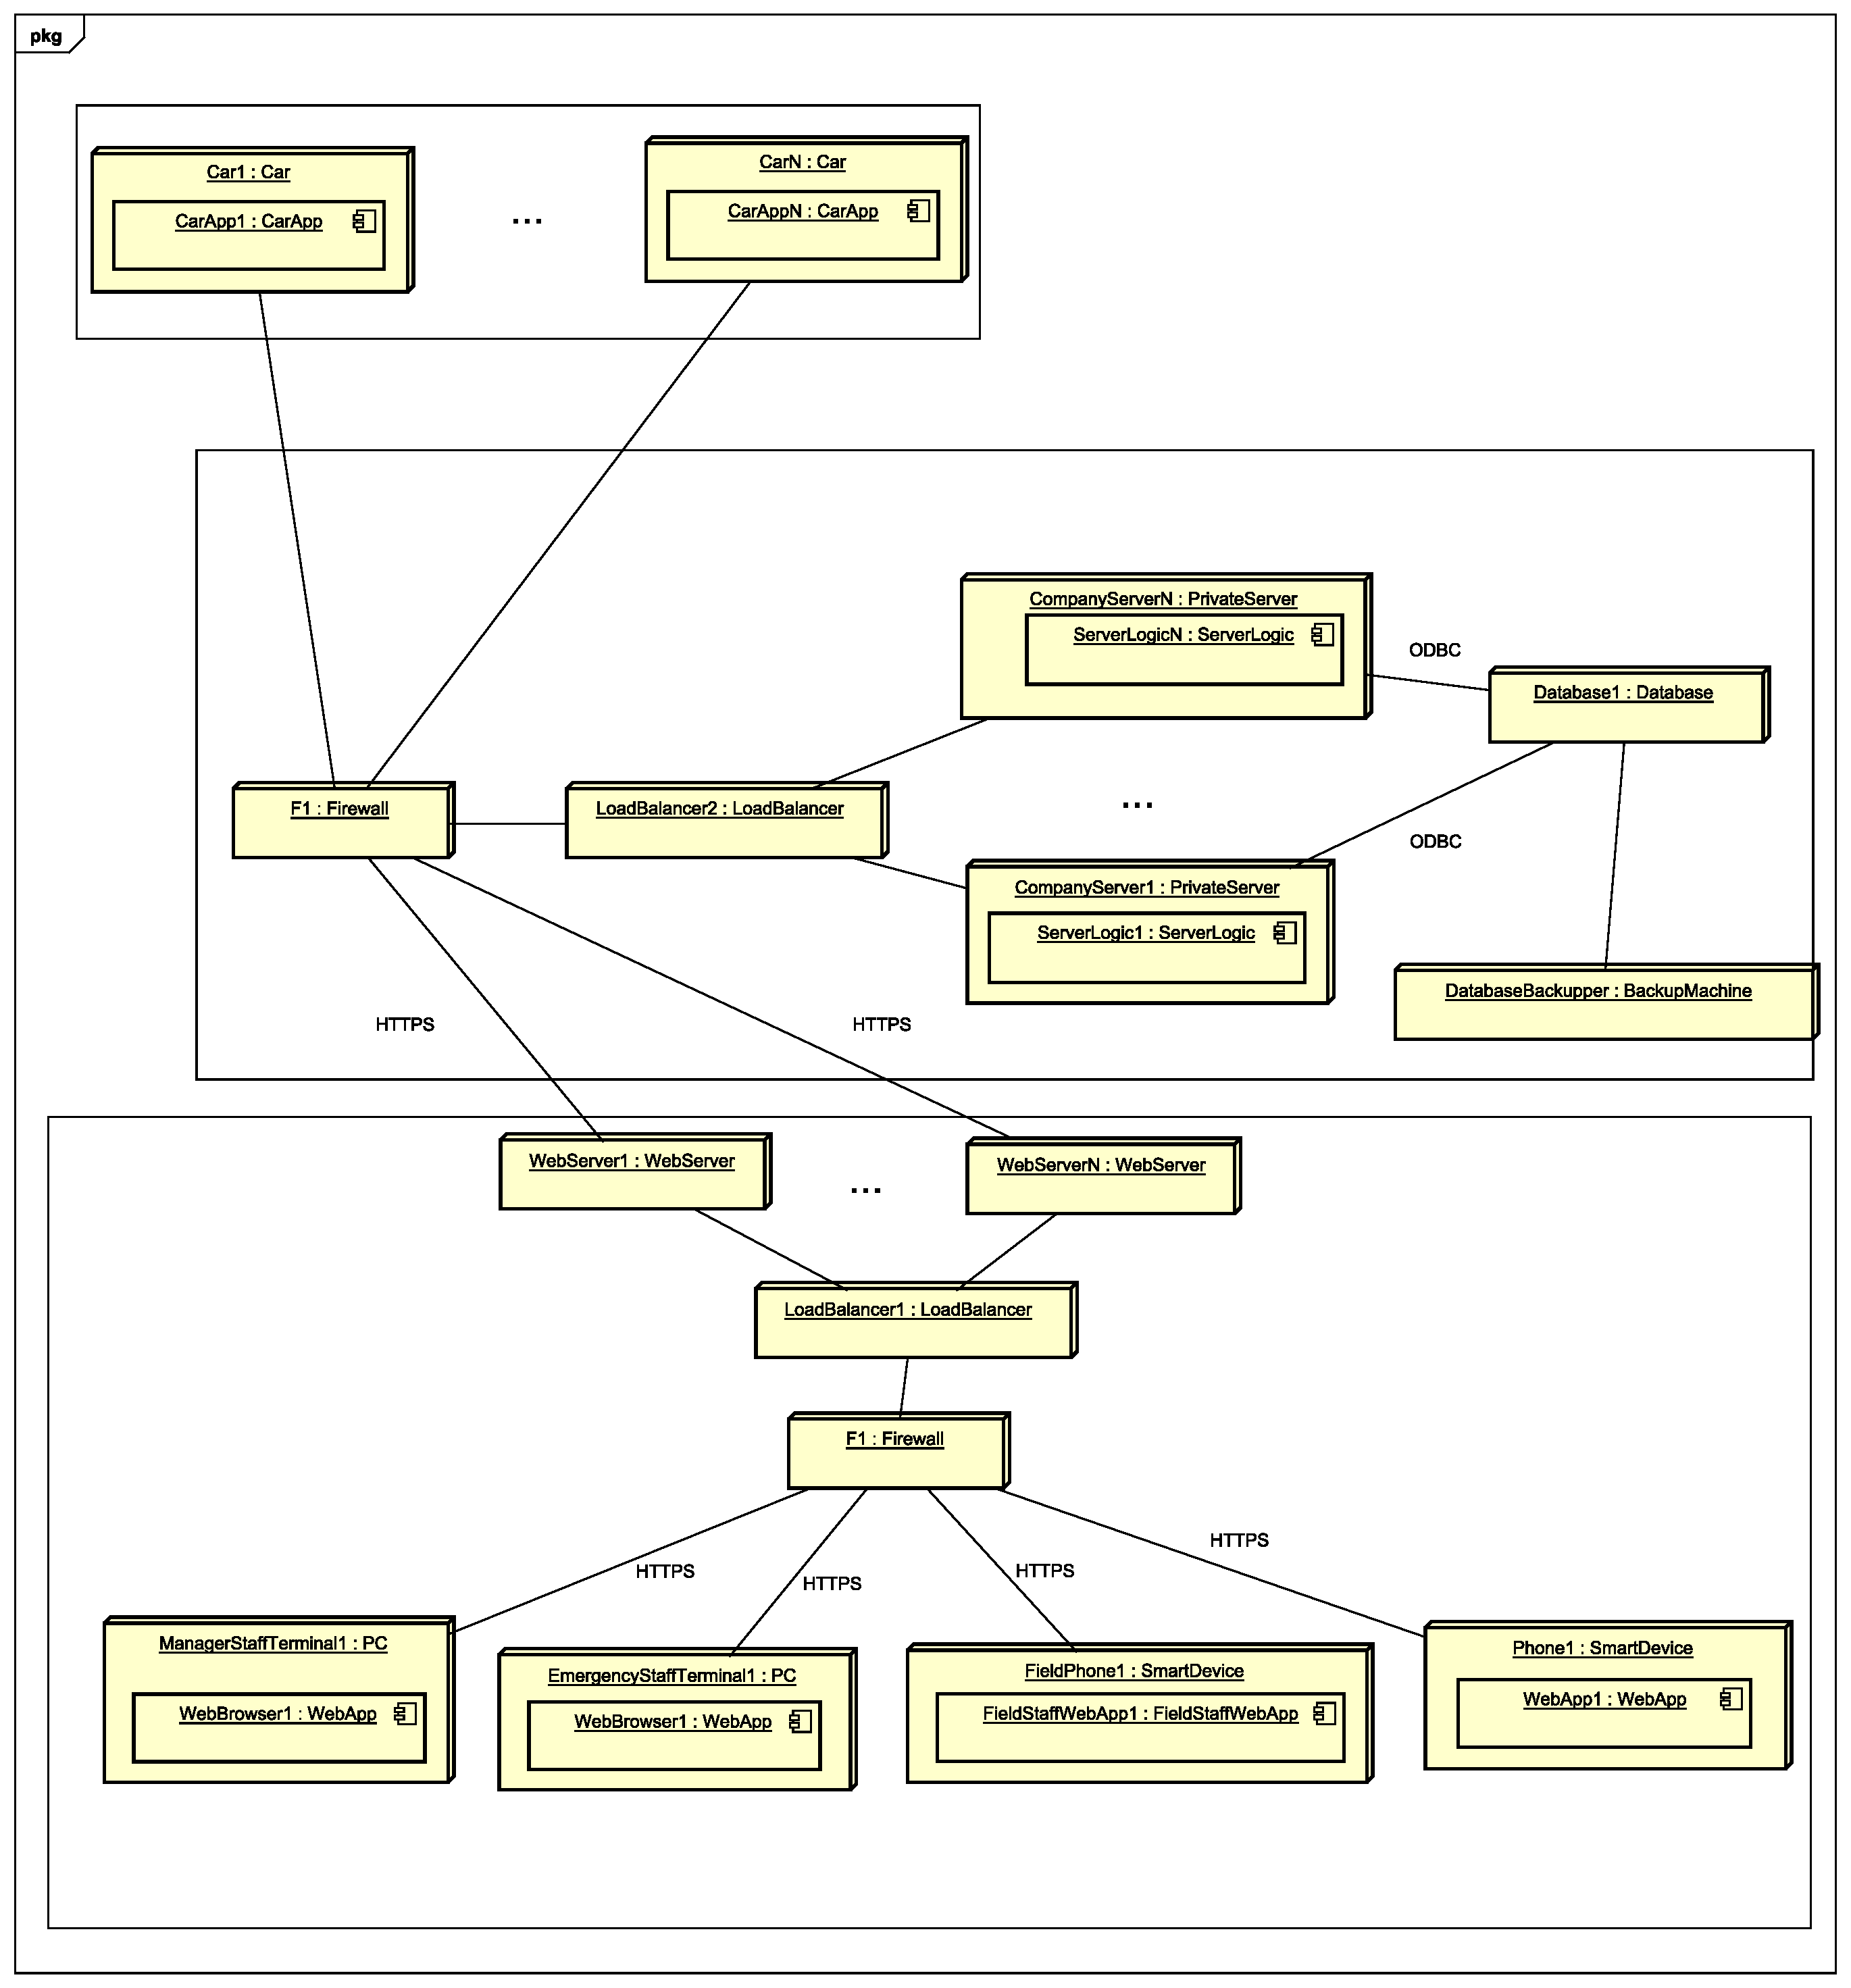
\includegraphics[scale=0.221875]{Deployment_Diagram.pdf}% "%" necessario
				\caption{Deployment Diagram}
			\end{figure}
	\begin{landscape}
	\subsection{Runtime view}%You can use sequence diagrams to describe the way components interact to accomplish specific tasks typically related to your use cases
		\begin{figure}[H]
				\centering
				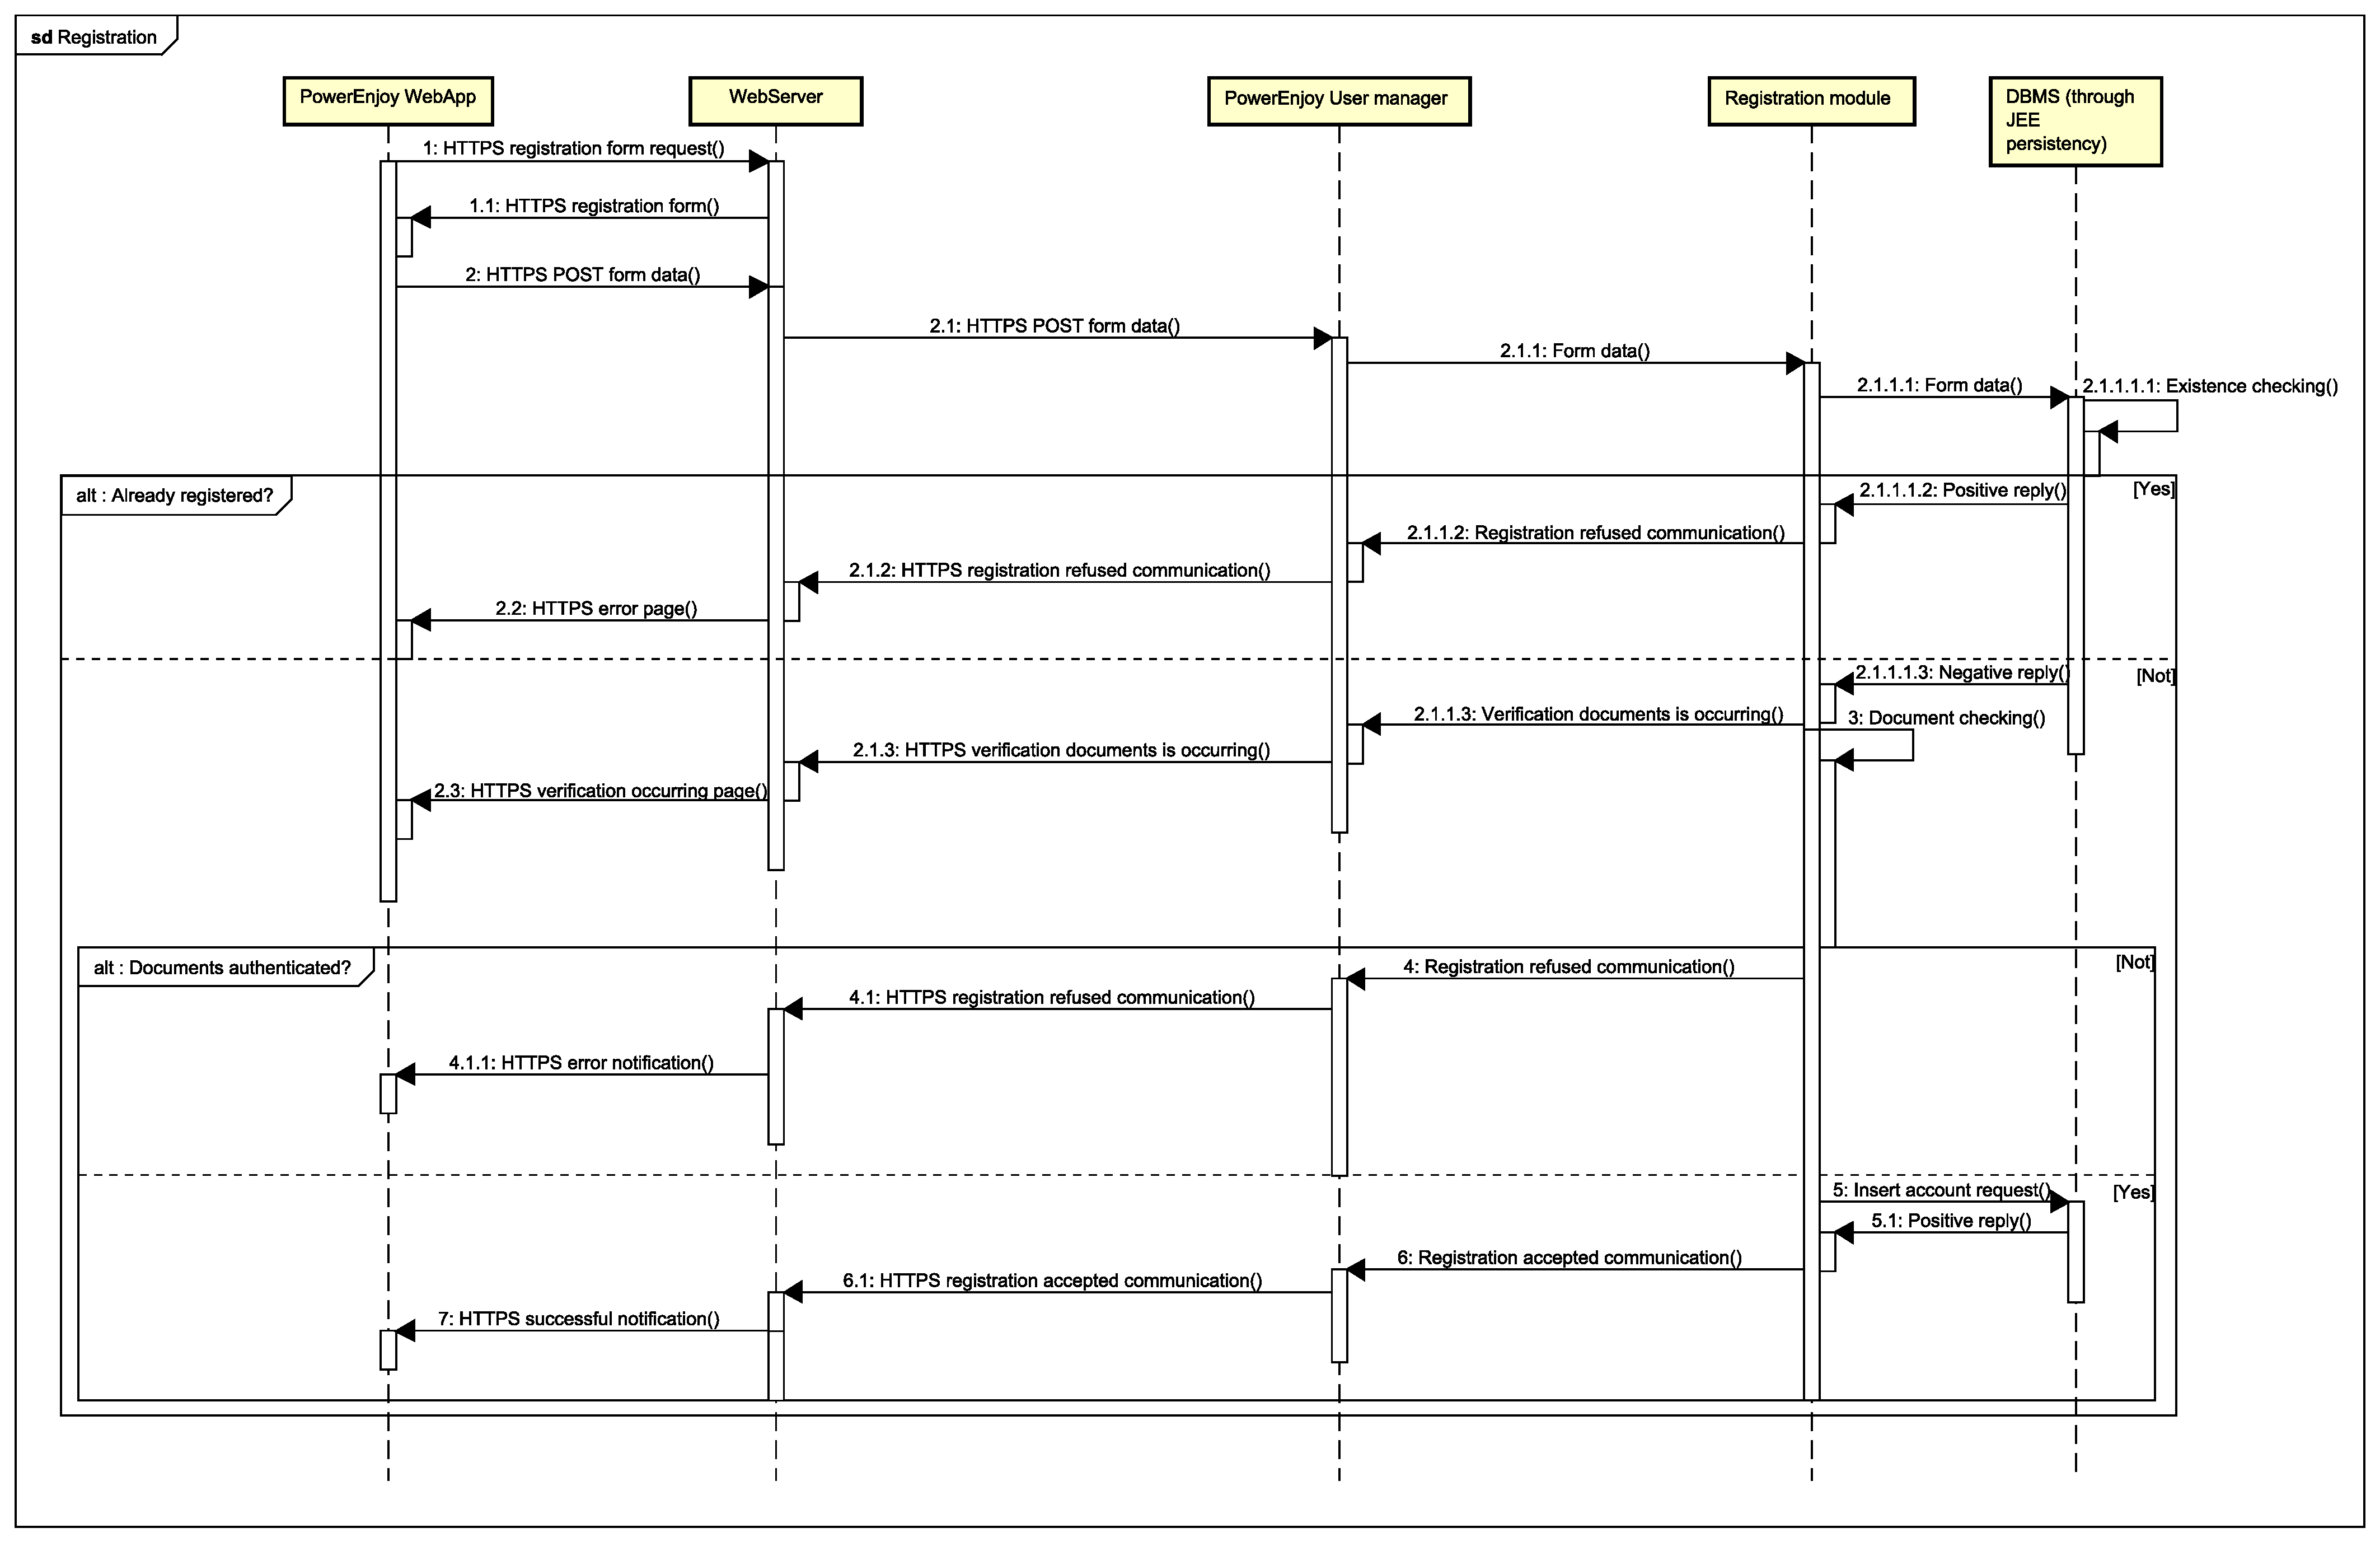
\includegraphics[scale=0.22]{./SequenceDiagrams/Registration/Registration.pdf}% "%" necessario
				\caption{Registration}
		\end{figure}
	\end{landscape}
		\subsubsection{Registration}
		In this sequence diagram we can see how the components work together in order to sign up an user to the service.
		For all the next communications the messages are transfered by a web server from mobile app to server's modules and viceversa. This is done for security and optimization purposes.
		First of all, the registration form is requested to the web server and the user fills it, then the proper data are sent to the registration module.
		These data are used to check the existence of the same account in the database.
		If the existence is verified, the new registration is denied and an error page is shown to the user. Otherwise the documents information to be checked are sent to the proper authority and it is shown to the user a page that tells him that the documents are being verified. At this point the flow is interrupted and every time the user tries to access the account, it will be shown the previous message.
		Once the authority reply reach the system, an action can be performed. If the documents are not verified, an error notification is sent to the user, otherwise a new account is added to the database and a positive notification is sent to the user.
		\subsubsection{Reservation}
		The following sequence diagram shows us how the components interact among them when a reservation request is caught by the user's interface.
		In accordance with the specifications designed in the RASD document, we can see that the user can not only see the cars close to its location, but also cars next to a specific address. To do this is requested a conversion from textual address to geolocation coordinates to the web server of Google. Obviously the user position is taken from geolocation sensor embedded in the mobile.
		For all the next communications the messages are transfered by a web server from mobile app to server's modules and viceversa. This is done for security and optimization purposes.
		Once the position is determined, it is sent to the map manager. It computes the area close to the position and requires to the database the informations of the free cars in that place.
		The informations are sent to the user's app and now he can read the cars features and choose one.
		This choice is sent to the reservation manager that creates a new reservation in the database and begins the timer.
		After that the confirmation is sent to the mobile app and the local timer begins.
		Leaning to Google servers, is calculated the route from user location to the chosen position, to allow him to get the car without difficulty.
	\begin{landscape}
		\begin{figure}[H]
				\centering
				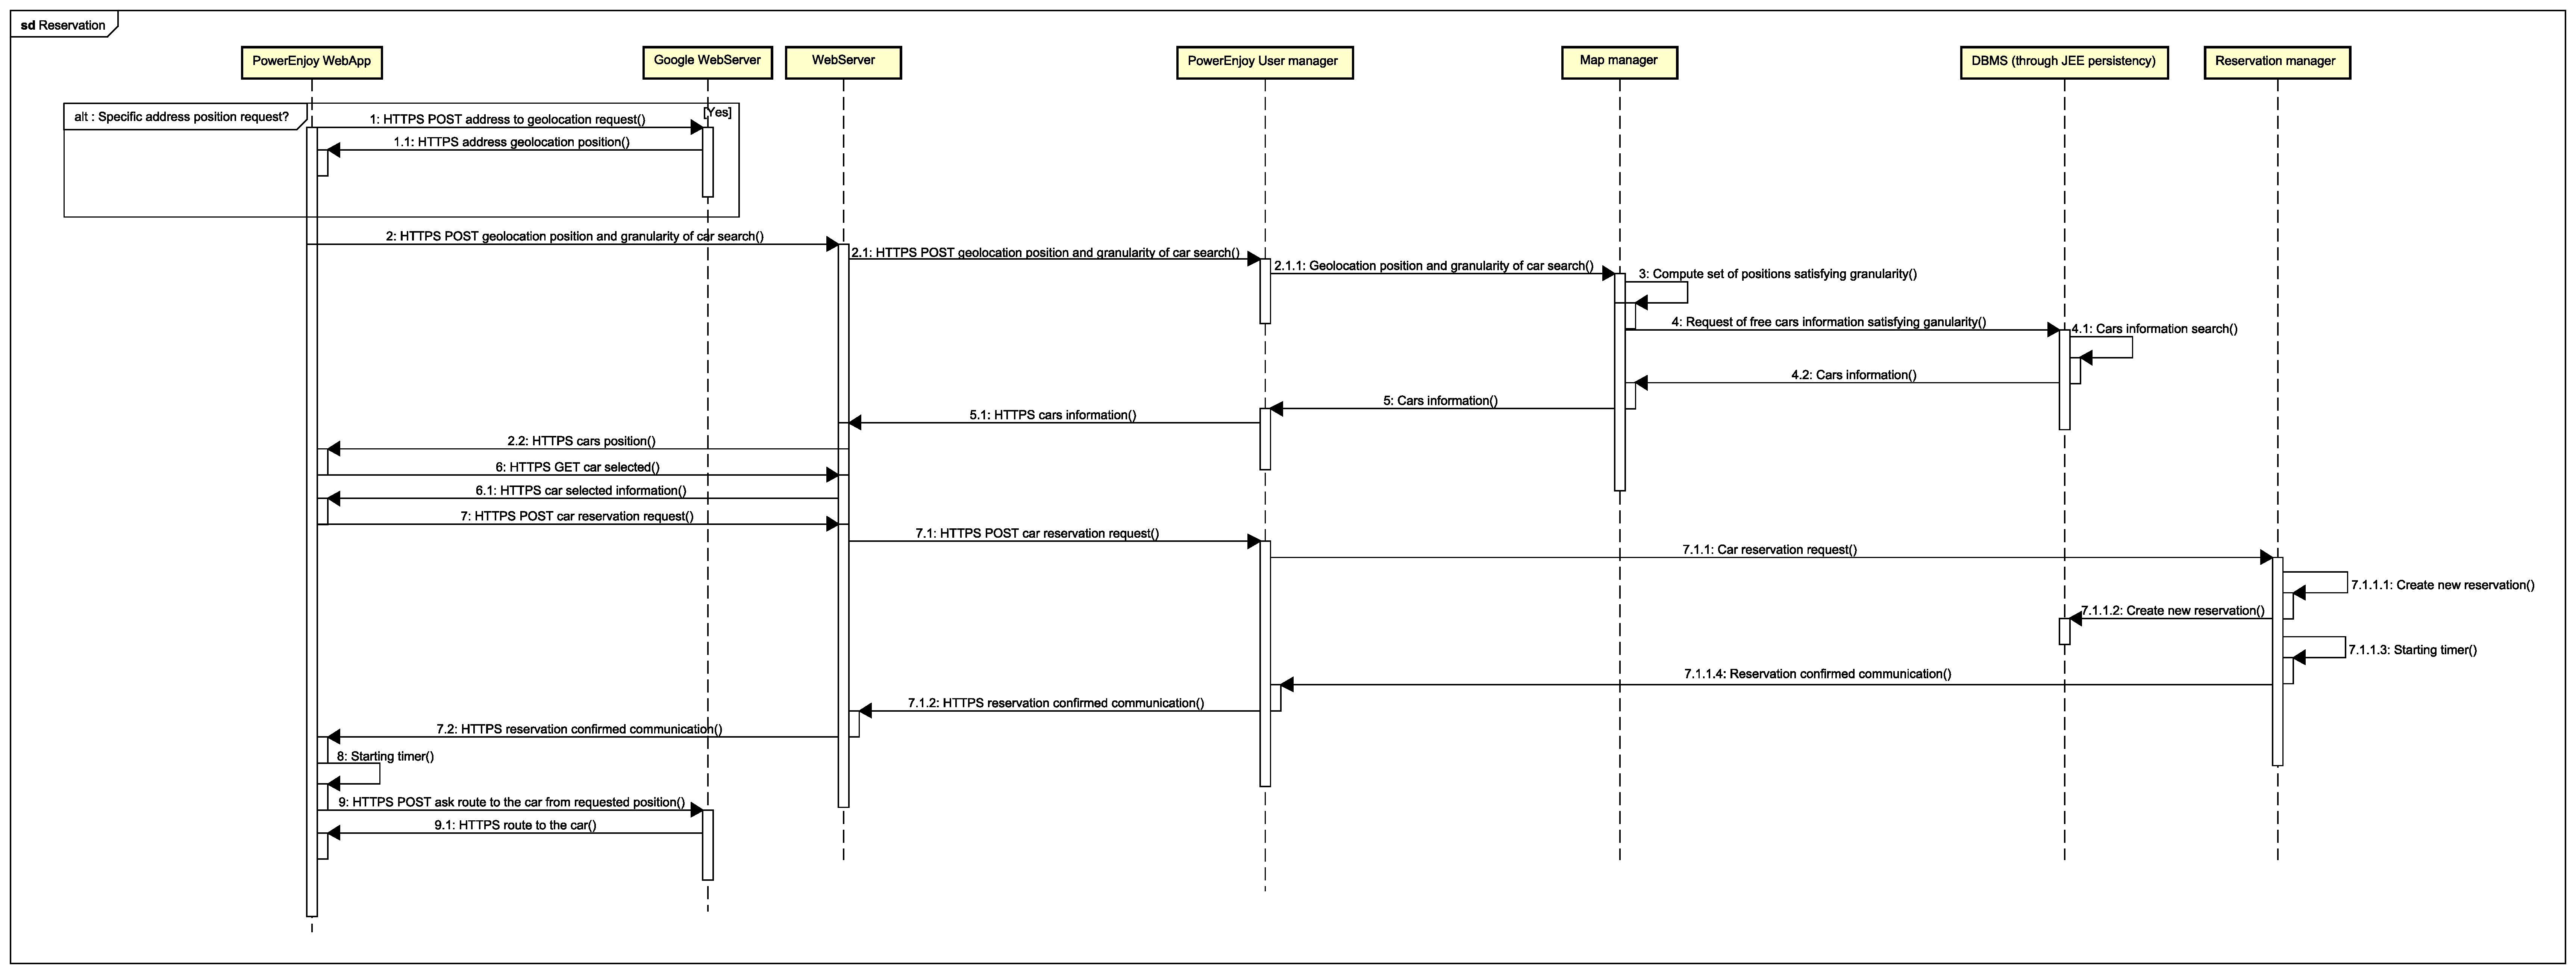
\includegraphics[scale=0.174]{./SequenceDiagrams/Reservation/Reservation.pdf}% "%" necessario
				\caption{Reservation}
		\end{figure}
	\end{landscape}
	\begin{landscape}
		\begin{figure}[H]
				\centering
				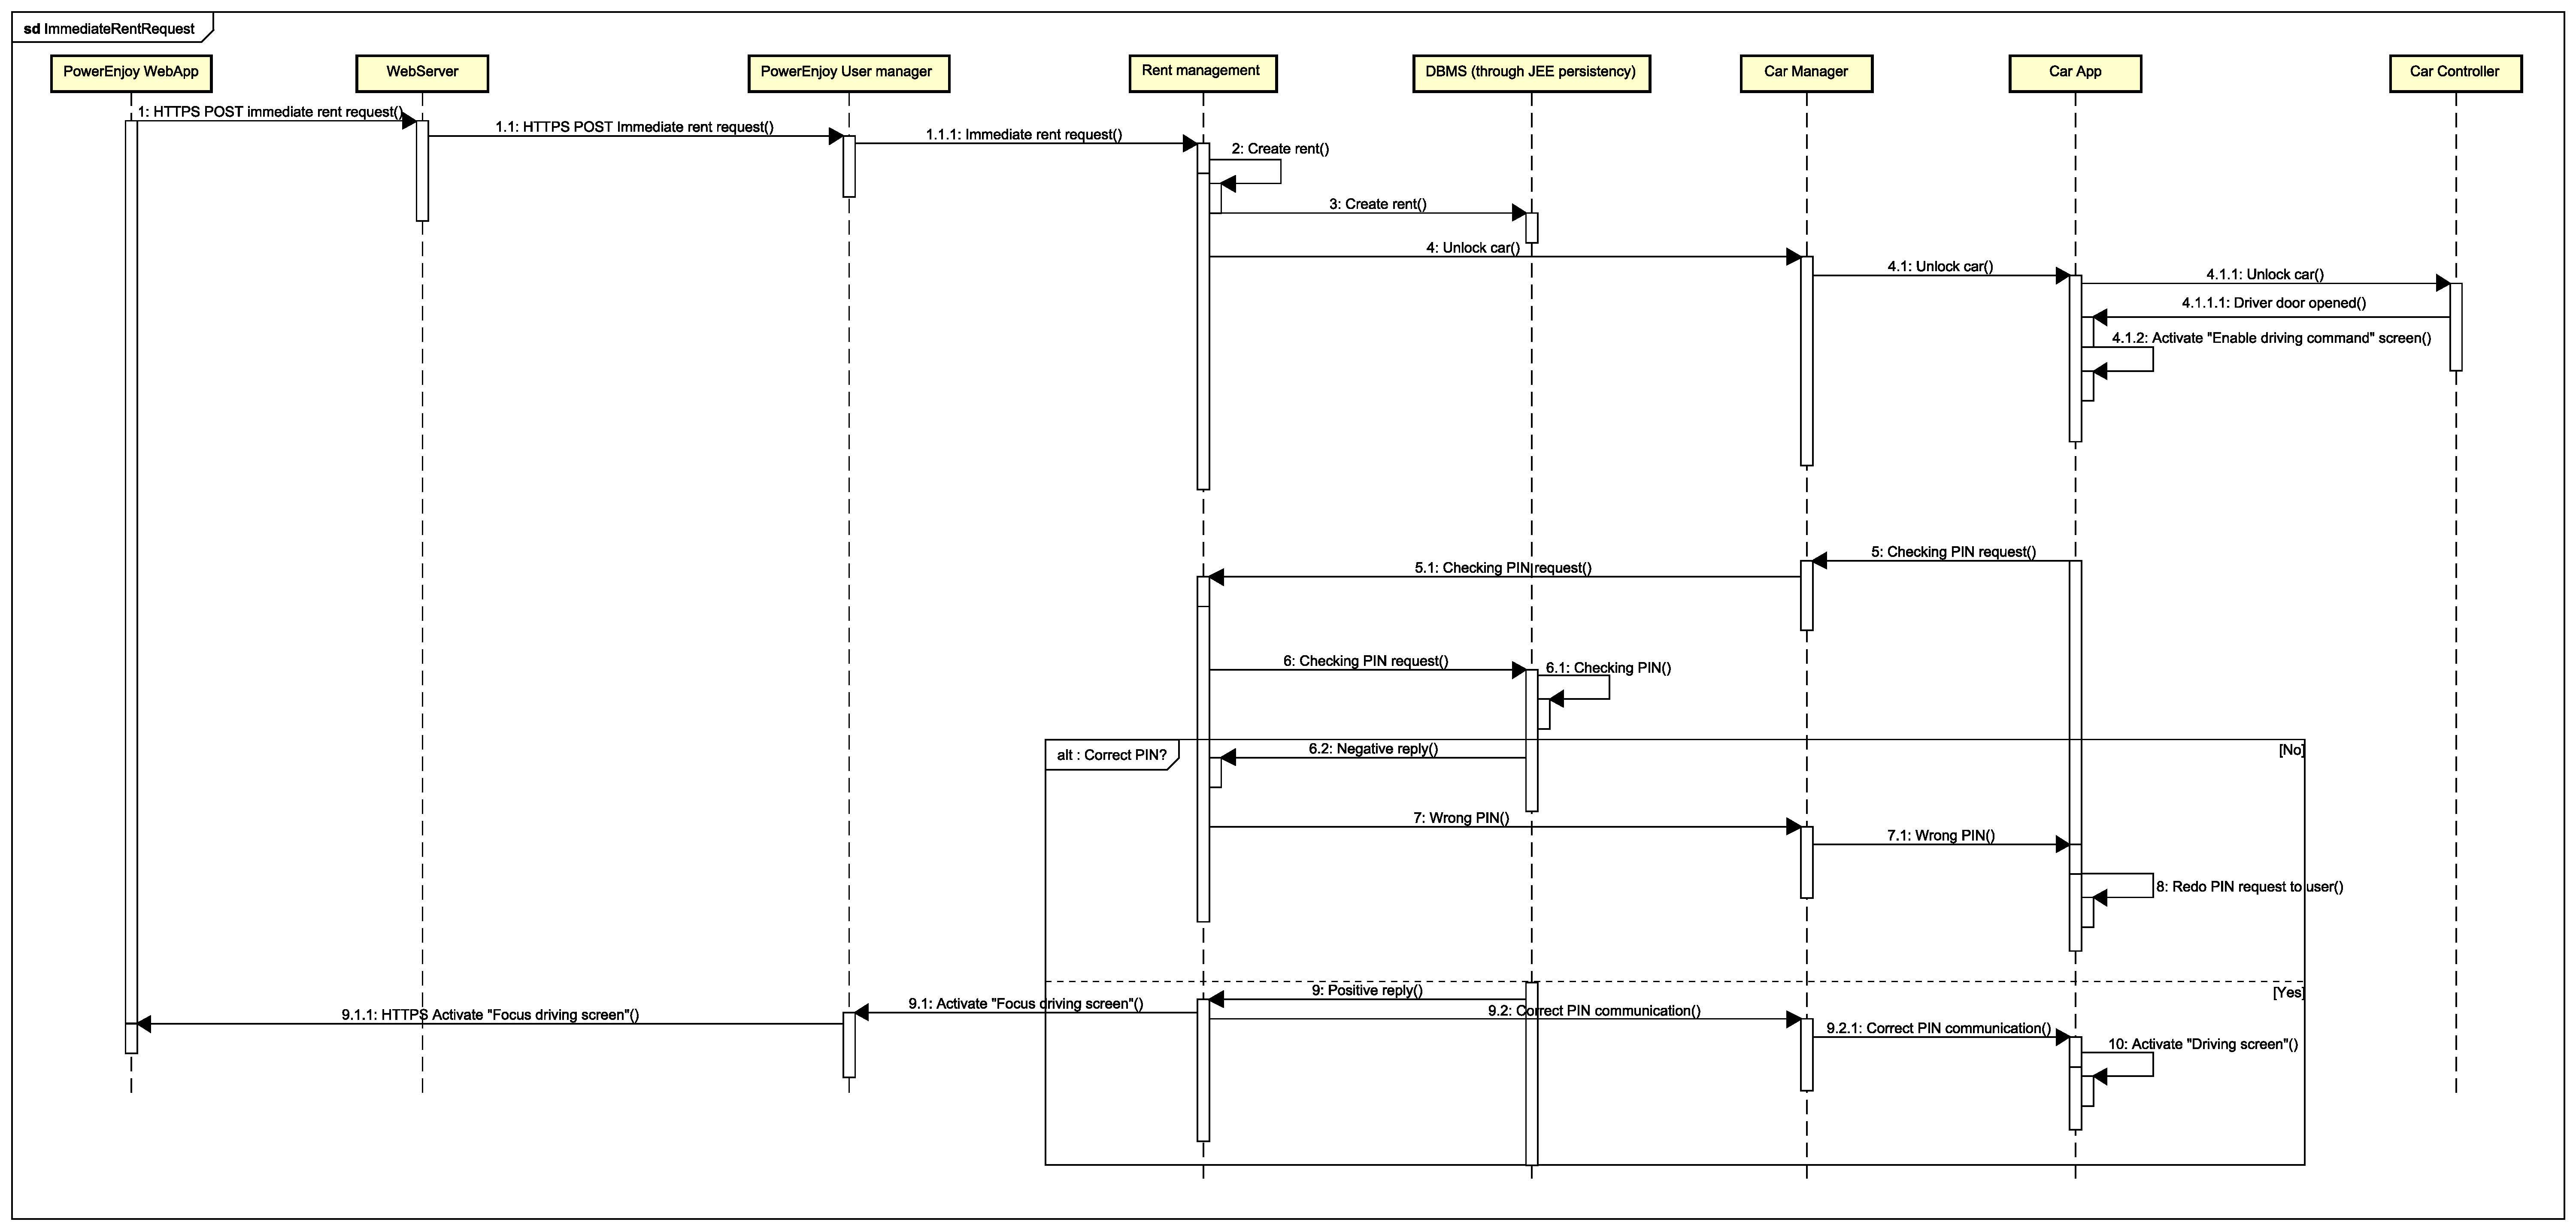
\includegraphics[scale=0.197]{./SequenceDiagrams/ImmediateRentRequest/ImmediateRentRequest.pdf}% "%" necessario
				\caption{Immediate Rent Request}
		\end{figure}
	\end{landscape}
		\subsubsection{Immediate Rent Request}
		In this other sequence diagram we can see more in detail the particular situation in which a user wants immediately rent a car when he is near it.
		For all the next communications the messages are transfered by a web server from mobile app to server's modules and viceversa. This is done for security and optimization purposes.
		The immedate rent request is sent to the rent manager that, after creates a rent in the database, asks to the car manager to unlock it. This module communicates with the car app and finally the operation is carried out by the car controller embedded in it. At the end of the operation, the appropriate screen is enabled on the car.
		At this point the flow is interrupted until the user fills the car screen with his correct PIN. After the insertion it is verified by a database query carried out by the rent manager. If the PIN is uncorrect, an error page is shown on the car screen and a new PIN insertion is requested, otherwise the "Focus driving screen" is activated on the mobile screen, the driving commands are enabled and the "Driving screen" is shown on the car. 
		\subsubsection{Money Saving Option}
		In this following sequence diagram the money saving option is described.
		We place ourselves in the situation in which the user is on the car and the rent is already began.
		The user fills a form on the car screen with the destination address. This address is converted immediately by google servers in a geolocation position.
		The user can now select the money saving option from the car screen. The request is sent to the rent manager and then to the BPM. The BPM computes the appropriate safe area where park the car and sends this information to the rent manager that communicates it to the car app.
		At this point the car app calculate the route to the destination using the own navigation system.
	\begin{landscape}
		\begin{figure}[H]
				\centering
				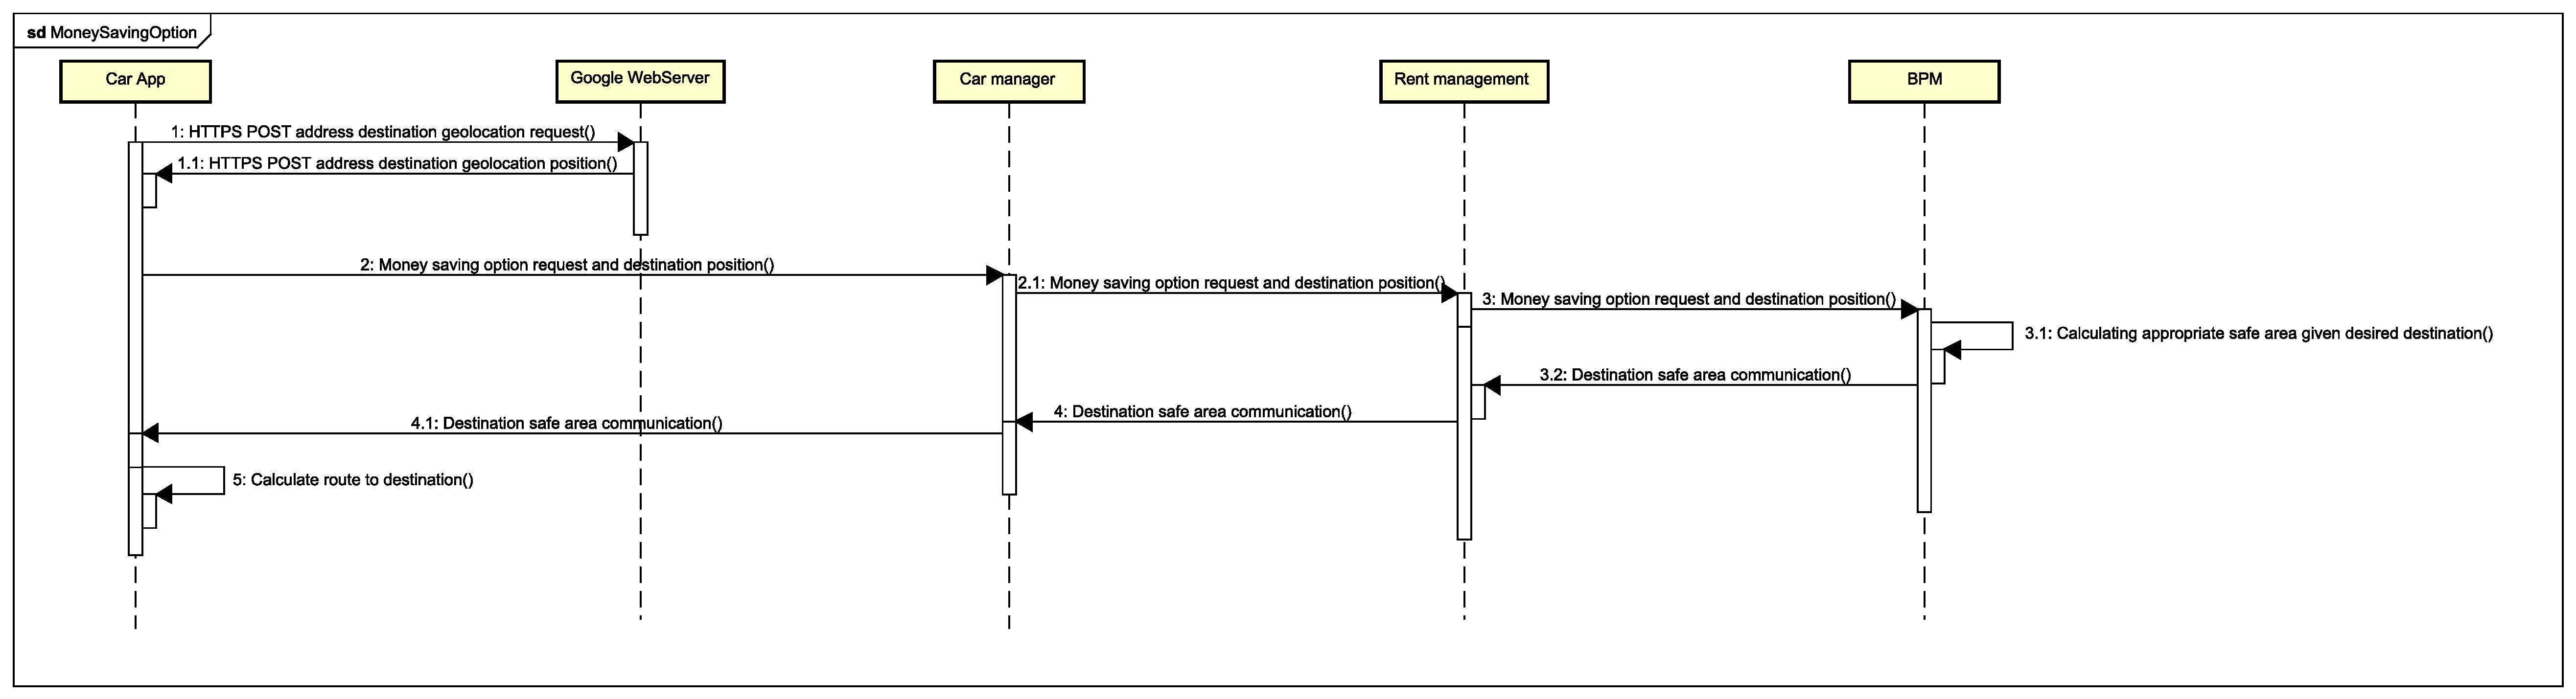
\includegraphics[scale=0.225]{./SequenceDiagrams/MoneySavingOption/MoneySavingOption.pdf}% "%" necessario
				\caption{Money Saving Option}
		\end{figure}
	\end{landscape}
	\subsection{Component interfaces}
	\subsubsection*{Google Map API}
		In order to offer the service, our system will be interfaced to external services. 
		Map services are offered by Google.
		Specifically our system will use the following Google services
	\paragraph {Maps JavaScript API}
		This component will provide maps functionalities. 
	\begin{itemize}
		\item map graphical representation.
		\item show markers
		\item show data on the map
	\end{itemize}
	\paragraph {Google Maps Geocoding API}
		Geocoding is the process of converting addresses, like a street address, into geographic coordinates. It will be used to position the map around a certain marker, prepare the car research request around a certain address.
		\par It will be used from \powerenjoy user application when he search to a specific address in the map.
	\paragraph {Google Places API Web Service}
		It works as the Geocoding API,  but it transforms remarkable places into geographic coordinates.
	\paragraph {Google Maps Geolocation API}
		The Google Maps Geolocation API returns a location and accuracy radius based on information about cell towers and WiFi nodes that the mobile client can detect. \par It will be used in order to detect the user position(Both \powerenjoy user and \fieldstaff users)  if the GPS signal of their smart device is not available.
	
	\paragraph {Google Maps Directions API}
		It is useful in order to Calculate directions among multiple locations.
		\par It will be used from \powerenjoy user in order to find the direction to their reserved car.
	
	\subsubsection*{Car interfaces}
	The car controller and the car app components offers crucial interfaces to the system. 
	\begin{itemize}
		\item \textbf{Sensor Data:} interface with the control unit in order to monitor the car sensors data.
		\item\textbf{Actuators:} interface to remote control the car actuators(for example menage doors locking).
		\item \textbf{Car Position:} access to the Car positioning system guarantees position coordinates monitoring.
		\item \textbf{Navigation API:} interaction with the car navigation system (for example we have to set the destination address of \moneysaving drive).
	\end{itemize}
	These interface will be done using the API offered by the car manufacturer.
	\subsubsection*{Smartphone Interfaces}
	Another crucial interface is the one with the \powerenjoy and \fieldstaff users smartphones.
		We will release two different versions of the application. One dedicated to \powerenjoy user and the other for \fieldstaff's smartphones. This application will be deployed using \fnurl{Phonegap build}{https://build.phonegap.com/}. This application will communicate to the web server via HTTPS requests.
	\paragraph{User Position Update}
			The running application should be also able to get the position of the user via Satellites, the Web App will be able to get it using the hardware positioning interfaces.
		\par The interface to the hardware positioning system will be done using API \fnurl{HTML5 geolocation}{http://www.w3schools.com/html/html5_geolocation.asp}.
	\subsubsection*{Document Validation API}
		In order to verify clients documents validity we will use external API. We will use \fnurl{idcheck.io RESTful API}{https://www.idcheck.io/offer/solutions/developers/}. Given the driving license and id photograph it allows to verify if they are falsified. This API uses RESTful and JSON.
	\subsubsection*{Registration API}
		This service will provide to the users the possibility to subscribe. This API will be used both from the Smartphone application and from the third party developers in order to register users to our service from an external service.
	\subsubsection*{Account API}
		This interface allows to \powerenjoy users the modification of their personal info. It is accessible from third party applications. Furthermore it allows the payment manager to lock the user account until he has pending payments. 
	\subsubsection*{Login API}
		This interface will provide the login functionality to \powerenjoy, management staff, fieleld staff, emergency staff and third party users to log into the service.
	\subsubsection*{Configuration}
	This is a set of interfaces that allow to the management \staff to change the service parameters.
	Specifically they are seven:
	\begin{enumerate} 
		\item \textbf{fare configuration:} it allows to change the price of the service and define new type of fares (for example fare per km). It is powered by a Domain specific language(DSL).
		\item \textbf{discount configuration:} it allows to change the service discount policies and to define new type of discounts. It is powered by a Domain specific language(DSL).
		\item \textbf{fee configuration:} it allows to change the fee price.
		\item \textbf{term of service configuration:} it allows to change the term of services. All the \powerenjoy users are notified of every new term are defined.
		\item\textbf{safe area configuration:} it allows to insert into the system the set of coordinates of new safe areas.
		\item \textbf{power plug configuration:} it allows to insert the coordinates of new power plug that can be used to charge \powerenjoy cars.
		\item \textbf{car configuration:} it allows to insert new cars into the system and start monitoring it.
	\end{enumerate}
	\subsection*{User app notification}
	This is a set of interfaces that allow the communication between different services and users manager services.
		\paragraph{Notification API}
		Is the API used to notify users manage of changes in terms of service. 
		\paragraph{Relocation Request}
		Is the Relocation Request calculated by BPM and sent to the \fieldstaff application.
		\paragraph{Maintenance Request}
		This inteface allows the communication between the Emergency Manager and the Field Staff manager. It allows to assign to the field staff maintenance requests. 
		\paragraph{Emergency task}
		This interface allow to notify the Emergency staff manager that a new emergency has to be queued for a certain Emergency staff user.
		\paragraph{Push notification API}
		this interface allow to make the notification possile it the Smartphone applications, it works via \fnurl{PUSH API }{https://developers.google.com/web/fundamentals/getting-started/codelabs/push-notifications/}by Google.
	\subsubsection*{DBMS API}
	Java EE persistency
	\subsubsection*{Calculate Price}
	this interface allows reservation management and rent management to calculate the respective price given the values that are managed by service configurator.	
	\subsubsection*{Reservation API}
	This interface allow users to make reservation. It works both for \powerenjoy app users and third party apps users.	
	\subsubsection*{Rent API}
	This interface allow users to make reservation. It works both for \powerenjoy app users and third party apps users.
	\subsubsection*{Payment Transaction}
	It is the interface that the payment manager offers and receives the price value of the transaction that it has to produce and the account info where to debit the money.
	\subsubsection*{Payment API}
	It is the payment service offered by \fnurl{Dwolla API}{https://developers.dwolla.com/}. This API works via HTTPS calls using Html POST requests encoded via JSON
	\subsubsection*{Recommend Destination}
	Is the the service offered by BPM that calculates the money saving destination given a certain rent. The destination is set in the car navigation system.
	\subsubsection*{Map Search API}
	Is the the service given by the map manager that provides the informations that the BMP needs in order to calculate relocation requests and money saving rent destinations.
	\subsubsection*{Availability Interface}
	Is the interfaces that provides the possibility to change the car availability according to the car state chart presented in the RASD document. 
	\subsubsection*{Map Updates}
	Is the service offered in order to send to clients the set of coordinates that they need to render over the map.
	\subsubsection*{User's Interfaces}
	It is the  set of interfaces that to allow maintain the current user session
	\begin{itemize}
		\item\textbf{FieldStaff Interface}
		\item\textbf{ManagementStaff Interface}
		\item\textbf{Emergency Staff Interface}
		\item\textbf{PowerEnjoyUser Interface}
		\item\textbf{Car interface}
	\end{itemize}
	\subsubsection*{Developer API}
	It is the interface that we offer to the third party developers in order to access to our system.
	
\subsection{Selected architectural styles and patterns} %Please explain which styles/patterns you used, why, and how
	\subsubsection{High Level Description}
	Our service will use a \textit{client/server} based architecture, 4-tier architecture. Client will be of three types, Smartphone clients, Web Browser clients, Car Clients.
	\paragraph{Smartphone Clients} these type of clients will run the application developed for \powerenjoy users and for \fieldstaff users. The smartphone clients will be thick clients because even  if the Business logic will be elaborated in the Private Servers, the native application will render all the data using JavaScript. 
		\par Specifically the applications will run on different platforms without rewriting code. It will be written using HTML5, JavaScript and CSS. We release the native application using Phonegap Build. 
		\par The application will be able to access to the client positioning system.
		\par The client will send request and receive data both from the Google maps services and from the web server.
	\paragraph{Web Browser Clients} these type of clients will run the service for the office \staff, it will allow the interface to the services of these two kind of clients. It will work using JavaScript, CSS, HTML5. 
	\paragraph{Car App Client} 
	This is the application that runs into \powerenjoy cars. It interfaces to the directly to the Private server via remote communication protocol. This client allows to manage the car remotely, to handle the \moneysaving requests and to set recommended destinations.
	\paragraph{Web Server}
	It is the interface between the Clients and the Private server. It manages the requests that come from the web clients. 
	\paragraph{Private Server}
	The private server runs all the business logic. It is developed using a \fnurl{microsevice architectural pattern}{https://en.wikipedia.org/wiki/Microservices}. This architecture guarantees that services are easy to be replaced and introduced. It also help the server maintainability, specifically if a component fails the error is only in its module
	\paragraph{DBMS}
	It supports the business logic processes providing data via SQL queries using ODBC protocol.
	\subsection{Other design decisions}
		\subsubsection{Programming Language}
			 For the implementation of PowerEnjoy system we choose Java as programming language. This choice is based on the following considerations:
			\begin{itemize}
				\item{Java is a very wide spread programming language, so we are sure that there will be more availability of skilled programmers in this technology.}
				\item{The system shall be developed on the Java EE platform, that ensures us large-scale, multi-tiered, scalable, reliable, and secure properties.}
			\end{itemize}
\section{Algorithm Design} %Focus on the definition of the most relevant algorithmic part 
	We are now going to present the most relevant algorithms of our application using some pseudo-code. The algorithms on which we focused our attention are those which manage the car search and the BPM logic.\\
	The syntax used to describe the algorithm stick to Python language, for its readability, but makes wide use of comments to better explain some functionalities without focusing too much on actual code.
	\subsection{Car search}
		The algorithm describes the behavior of the car search function. This function performs a search of the cars belonging to the circle having "location" as center and "radius" as radius. This is done by executing a DBMS query. Finally the result is returned as an array of objects.\\
		In the code is present an SQL query to give an idea of how the DBMS capabilities are exploited in order to perform some parts of the algorithm.
		\clearpage
		\code{Car search:}{./Algorithm/CarSearch/car_search.py}
	\subsection{BPM}
		This algorithm cover the main functionalities of the BPM component:
		\begin{itemize}
			\item assigning relocations to field staff users
			\item recommending destination for money saving options
		\end{itemize}
		In order to accomplish so, a sequence of intermediate steps is repeated in a cycle every 25 minutes, since the field staff reaction time is supposed to be 15 minutes in the domain assumptions.
		These steps include the computation of a relocation priority for cars (to relocate away) and safe areas / power plug slots (to relocate in), which will be used to select the relocations by picking the car and the safe area with highest priority, and assigning that relocation to field staff user with lower amount of queued tasks.\\\\
		NOTE: the relocation priority for cars and safe areas is computed as a number, whose value decreases as the priority increases.
		Two special values are reserved for battery charge related relocations, which have maximum priority:
		\begin{itemize}
			\item{ PRIORITY\_HIGH 	     (-1) 	for car with empty battery parked in a safe area }
			\item{ PRIORITY\_HIGHEST (-2) 	for car with empty full battery parked in a power plug slot }
		\end{itemize}
		For cars parked in safe area, the priority is computed looking at two different criteria,  weighted in different ways:
		\begin{enumerate}
			\item{ Cars parked in over-parked city zones should be relocated with priority proportional to the car excess in the zone. \\
					Weighted by IMPORTANCE\_HIGH (1e10) to have maximum impact over the priority. }
			\item{ Among the safe areas in same city zone, cars parked in almost-full safe areas have precedence. This is represented by the safe area load factor (parked cars / safe area capacity). \\ 
			Weighted by IMPORTANCE\_LOW (1e5) to have impact over the priority only when safe areas are in the same city zone. }
		\end{enumerate}
		For example, consider 3 cars:
		\begin{enumerate}
			\item{ parked in safe area with load factor 0.75, in city zone with +20 cars w.r.t. the optimal car number: \\
			Computed priority is:\\
			 $
			 priority = {1 \over \Delta cars} \times importance\_high + load\_factor \times importance\_low = 500075000
			 $}
			\item{ parked in safe area with load factor 0.1, in city zone with +100 cars w.r.t. the optimal car number.\\
			Computed priority is:\\
			 $
			 priority = {1 \over \Delta cars} \times importance\_high + load\_factor \times importance\_low = 100010000
			 $ }
			\item{ car with \textbf{empty battery} parked in safe area with load factor 0.05, in city zone with -20 cars w.r.t. the optimal car number.\\
			Computed priority is:\\
			 $
			 priority = -1,  \text{because is a special case}
			 $}
		\end{enumerate}
		The cars will be sorted by relocation\_priority in descendent order, thus relocated in order: [3], [2], [1].\\   
		\code{BPM: }{./Algorithm/bpm.py}
\section{User Interface Design}%Provide an overview on how the user interface(s) of your system will look like; if you have included this part in the RASD, you can simply refer to what you have already done, possibly, providing here some extensions if applicable.
		\subsection{PowerEnjoy user}
			\subsubsection{UX diagrams}
				\begin{figure}[H]
					\centering
					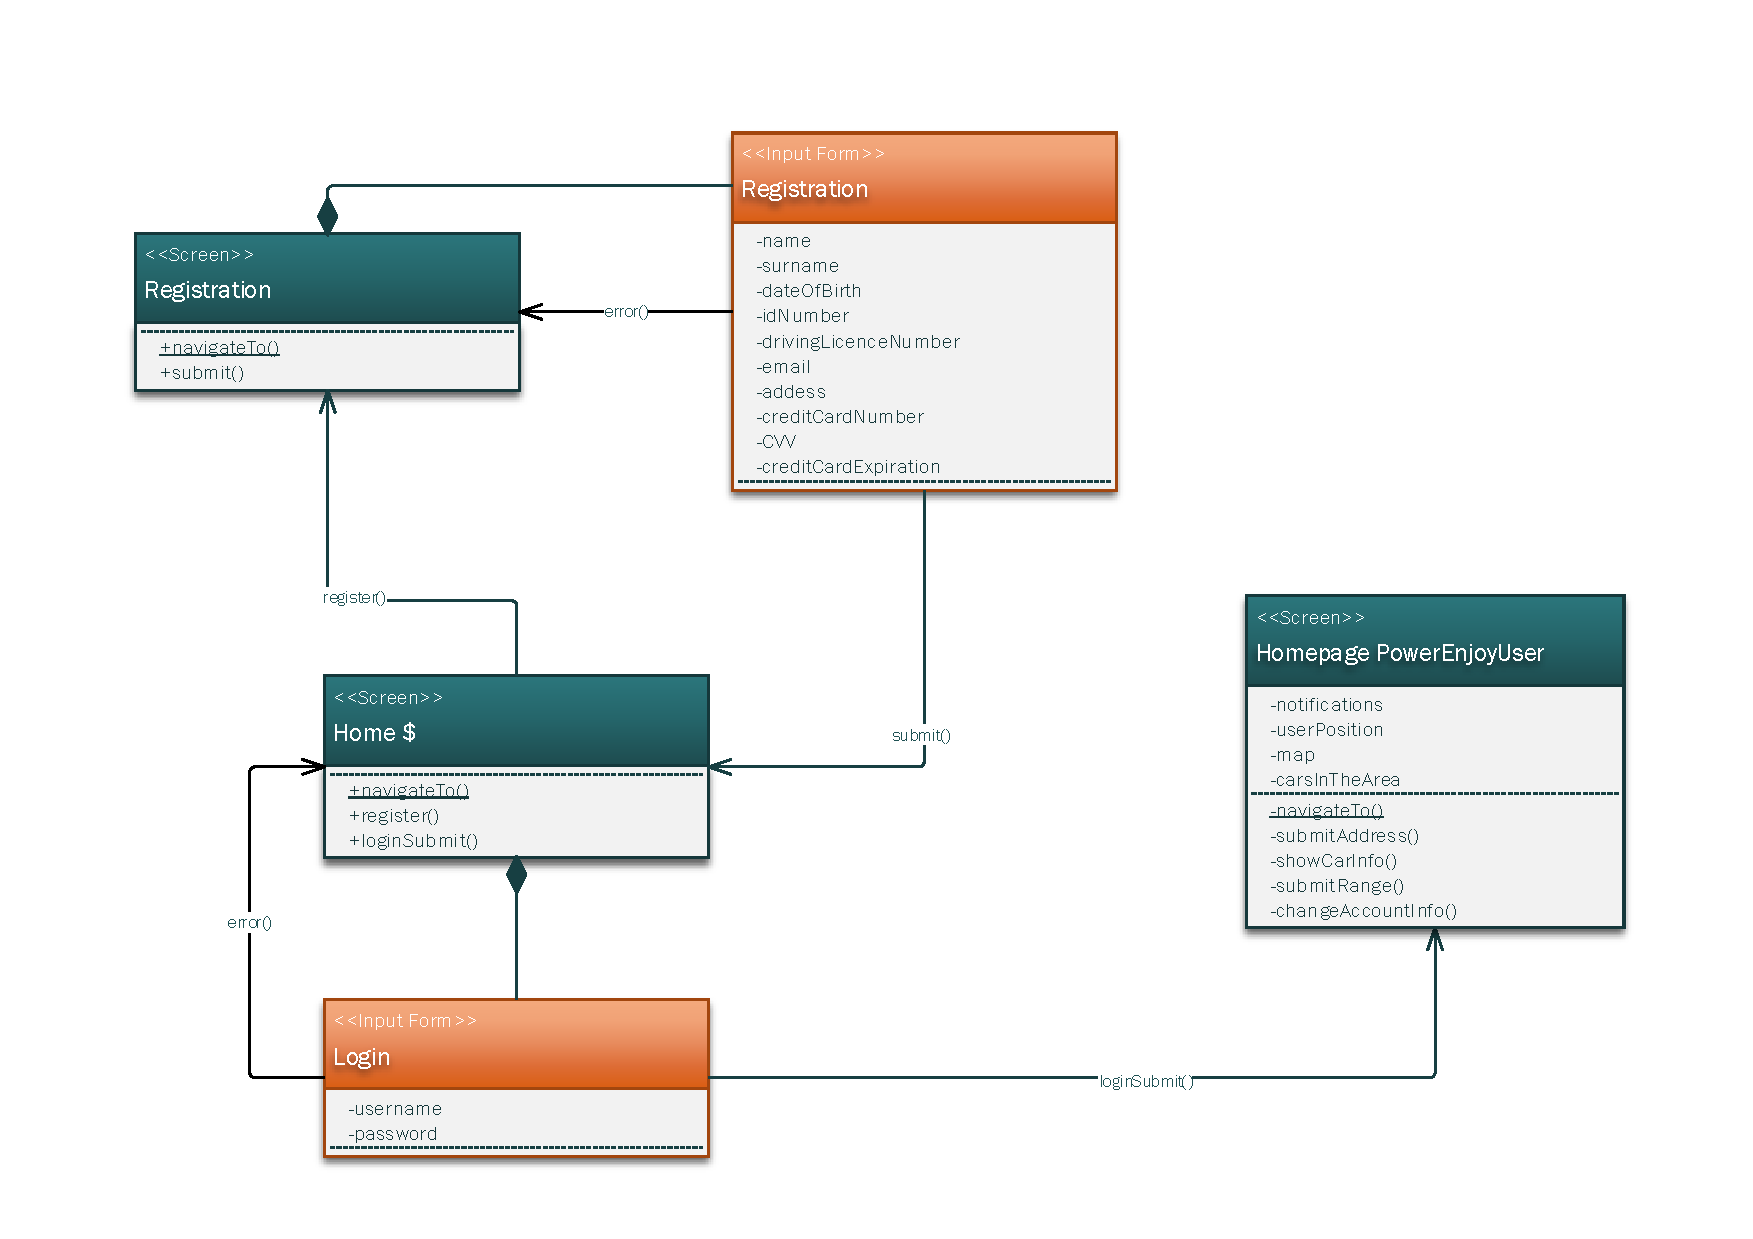
\includegraphics[scale=0.55]{./UXDiagrams/User/Login/UXDiagramRegistrationAndLoginUser.pdf}% "%" necessario
					\caption{Registration \& Login}
				\end{figure}
				\begin{landscape}
					\begin{figure}[H]
						\centering
						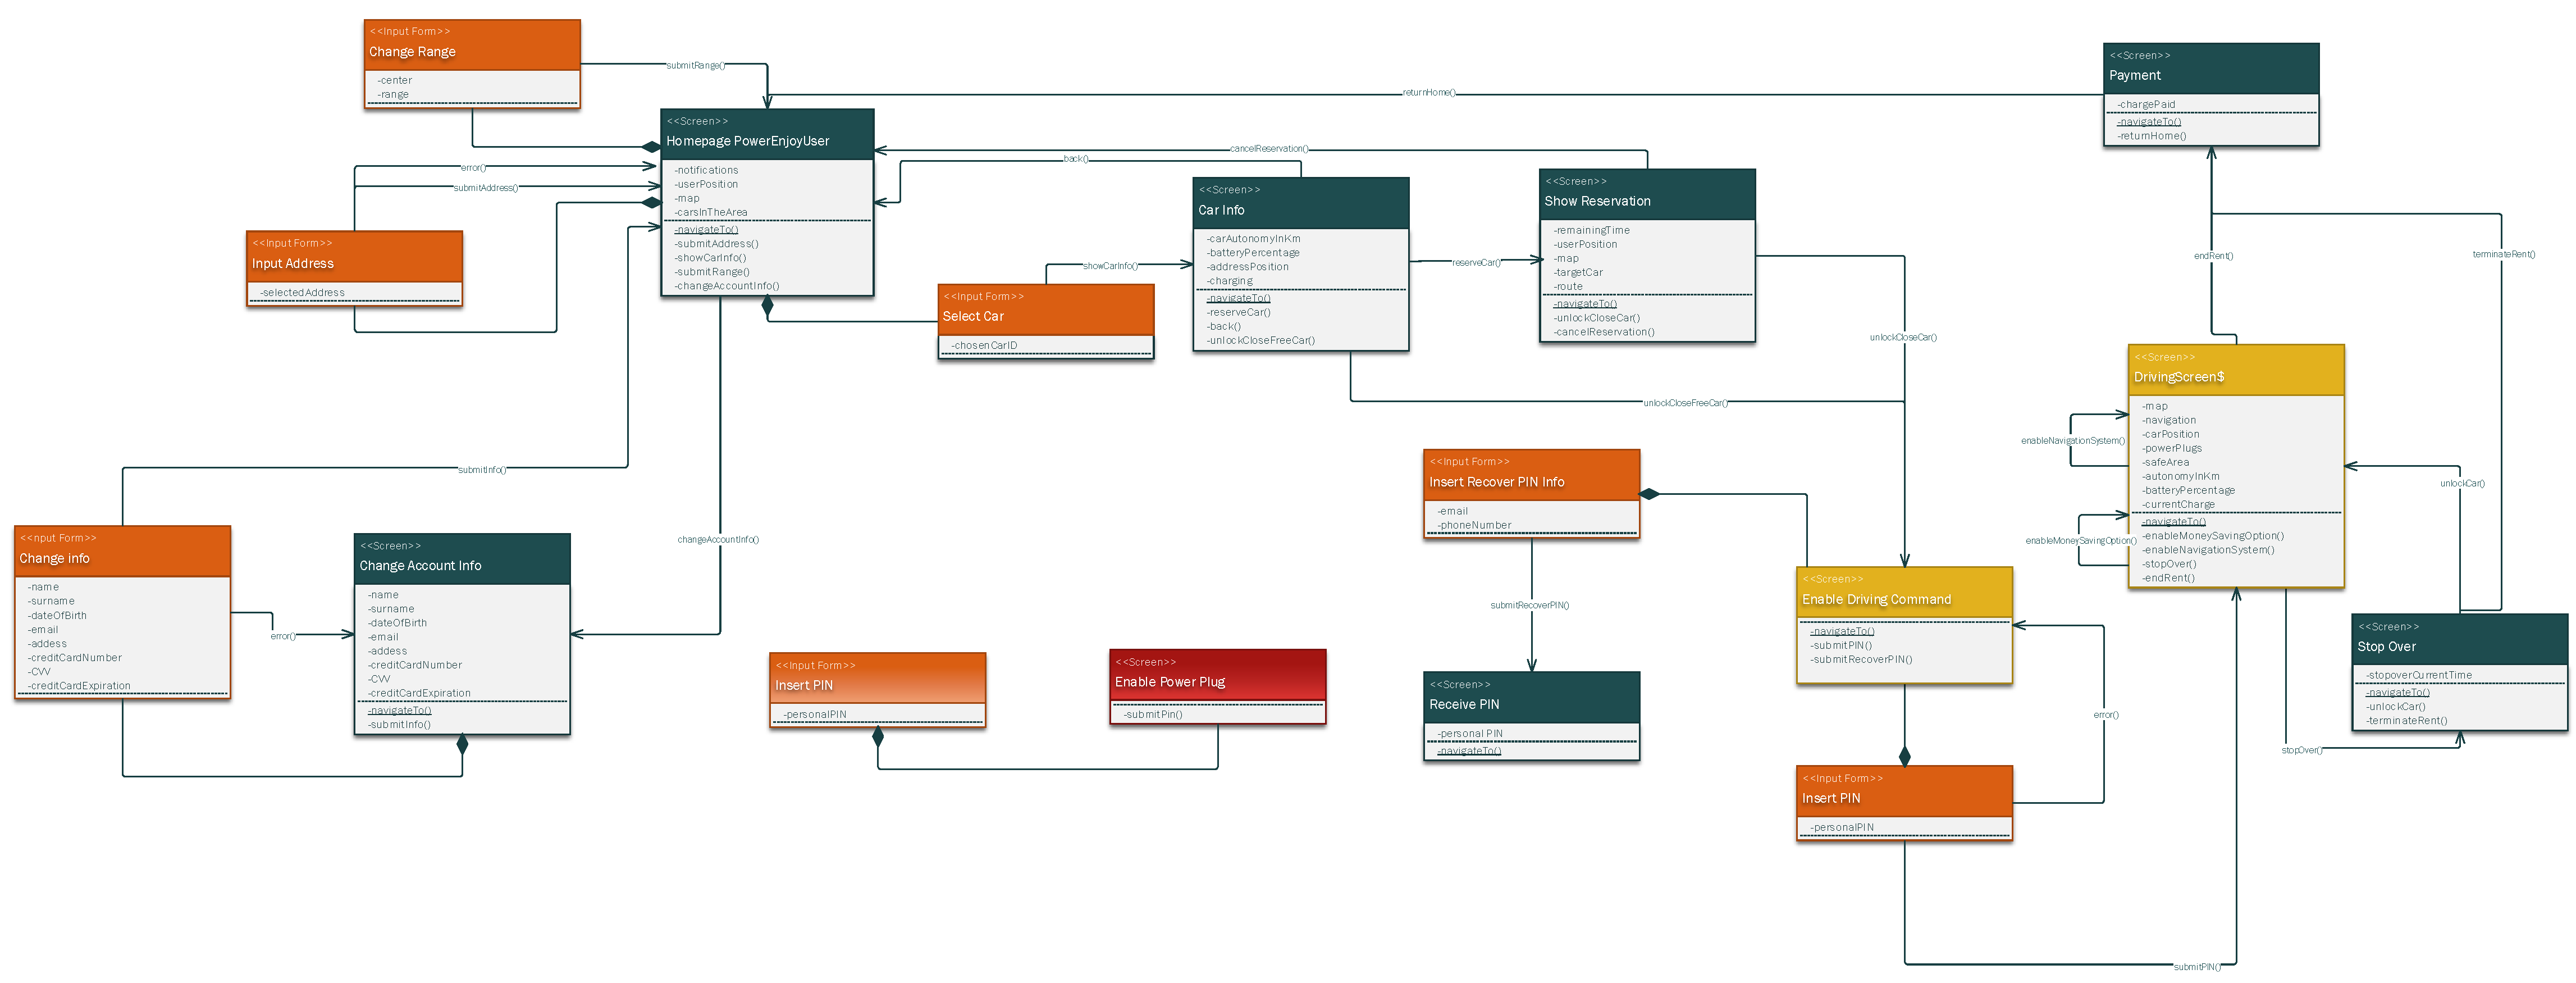
\includegraphics[scale=0.26]{./UXDiagrams/User/ReservationAndRent/UXDiagramPowerEnjoyUserSchermoCellulareAuto.pdf}% "%" necessario
						\caption{Reservation \& Rent}
					\end{figure}
				\end{landscape}
			\subsubsection{Mockups}
				\begin{figure}[H]
					\centering
					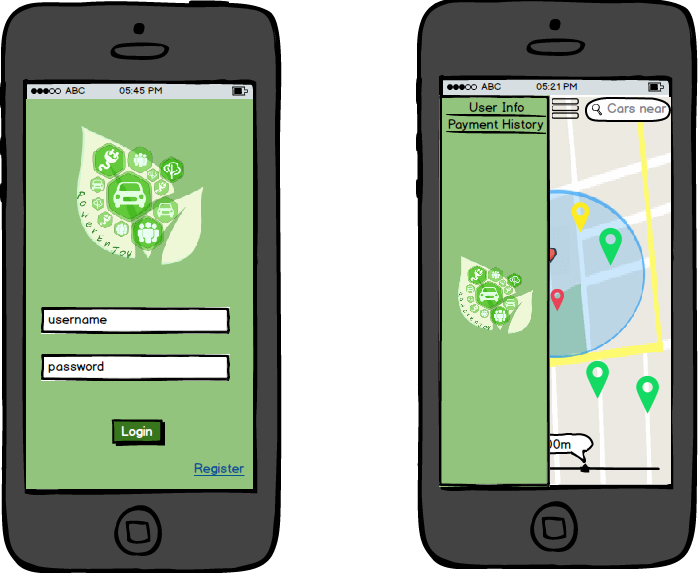
\includegraphics[scale=0.4]{./Mockups/powerEnjoyUser/login+menu.png}% "%" necessario
					\caption{Login \& Menu}
				\end{figure}
				\begin{figure}[H]
					\centering
					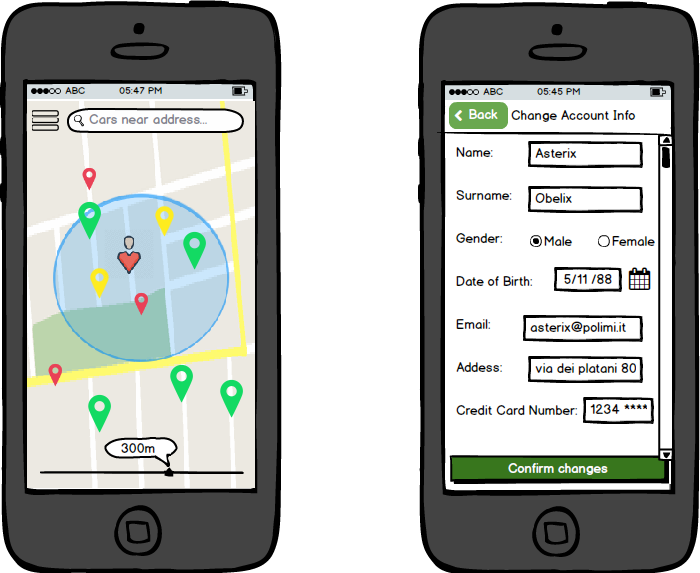
\includegraphics[scale=0.4]{./Mockups/powerEnjoyUser/powerEnJoy+accountInfo.png}% "%" necessario
					\caption{PowerEnJoy \& Account Info}
				\end{figure}
				\begin{figure}[H]
					\centering
					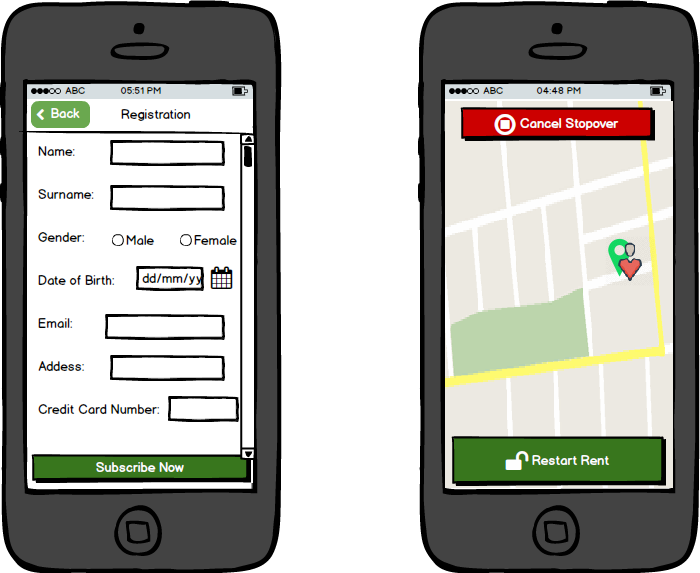
\includegraphics[scale=0.4]{./Mockups/powerEnjoyUser/singUp+stopOver.png}% "%" necessario
					\caption{Registration \& Stopover}
				\end{figure}
				\begin{figure}[H]
					\centering
					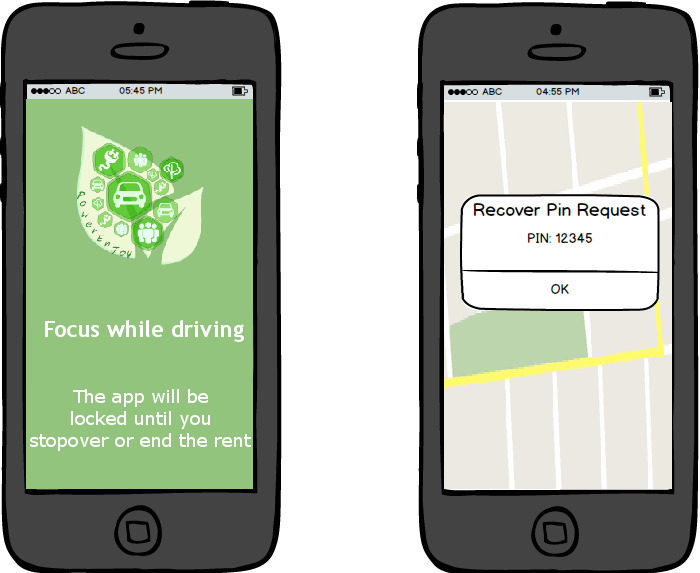
\includegraphics[scale=0.4]{./Mockups/powerEnjoyUser/focusDriving+requestPin.png}% "%" necessario
					\caption{Focus Driving\& Request Pin}
				\end{figure}
				\begin{figure}[H]
					\centering
					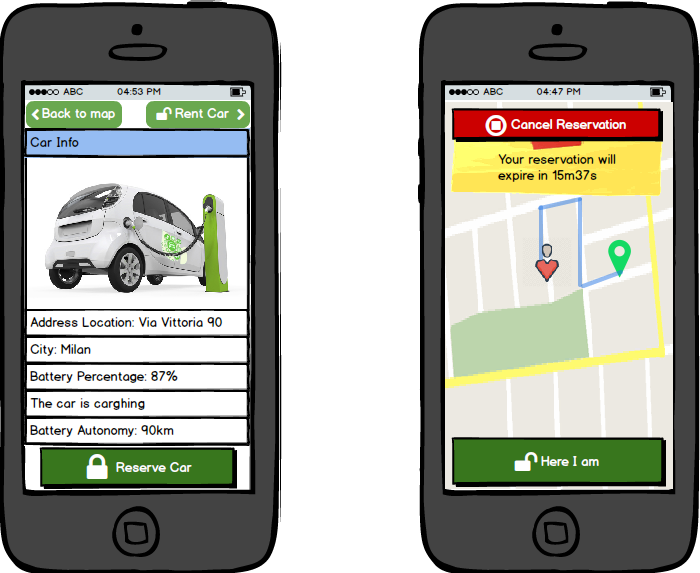
\includegraphics[scale=0.4]{./Mockups/powerEnjoyUser/carInfo+reservation.png}% "%" necessario
					\caption{Car Info \& Reservation}
				\end{figure}
		\begin{landscape}
			\subsection{Car}
				\subsubsection{Mockup}
					\begin{figure}[H]
						\centering
						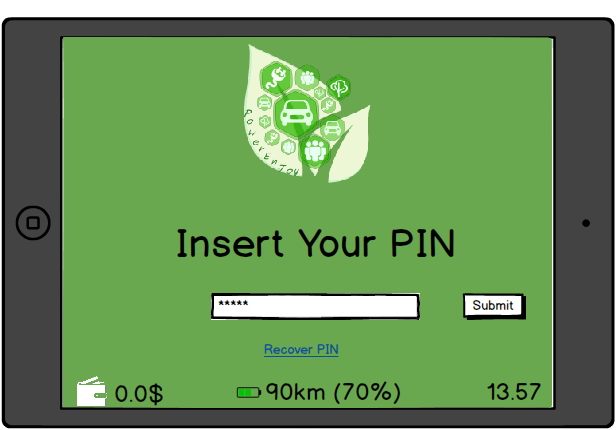
\includegraphics[scale=0.6]{./Mockups/Car/insertPIN.png}% "%" necessario
						\caption{PIN Insertion}
					\end{figure}
					\begin{figure}[H]
						\centering
						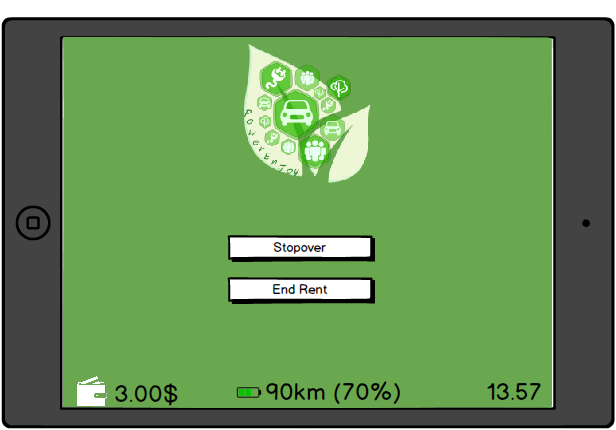
\includegraphics[scale=0.6]{./Mockups/Car/Stopover-endrent.png}% "%" necessario
						\caption{Stopover or End Ret Screen}
					\end{figure}
					\begin{figure}[H]
						\centering
						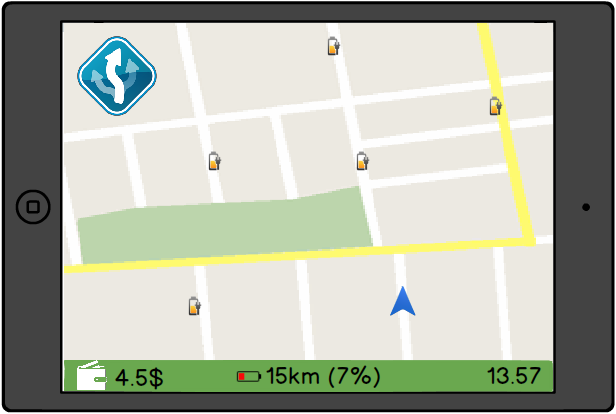
\includegraphics[scale=0.6]{./Mockups/Car/carscreen.png}% "%" necessario
						\caption{driving screen}
					\end{figure}
			\end{landscape}
		\subsection{FieldStaff}
			\subsubsection{UX diagrams}
				\begin{figure}[H]
					\centering
					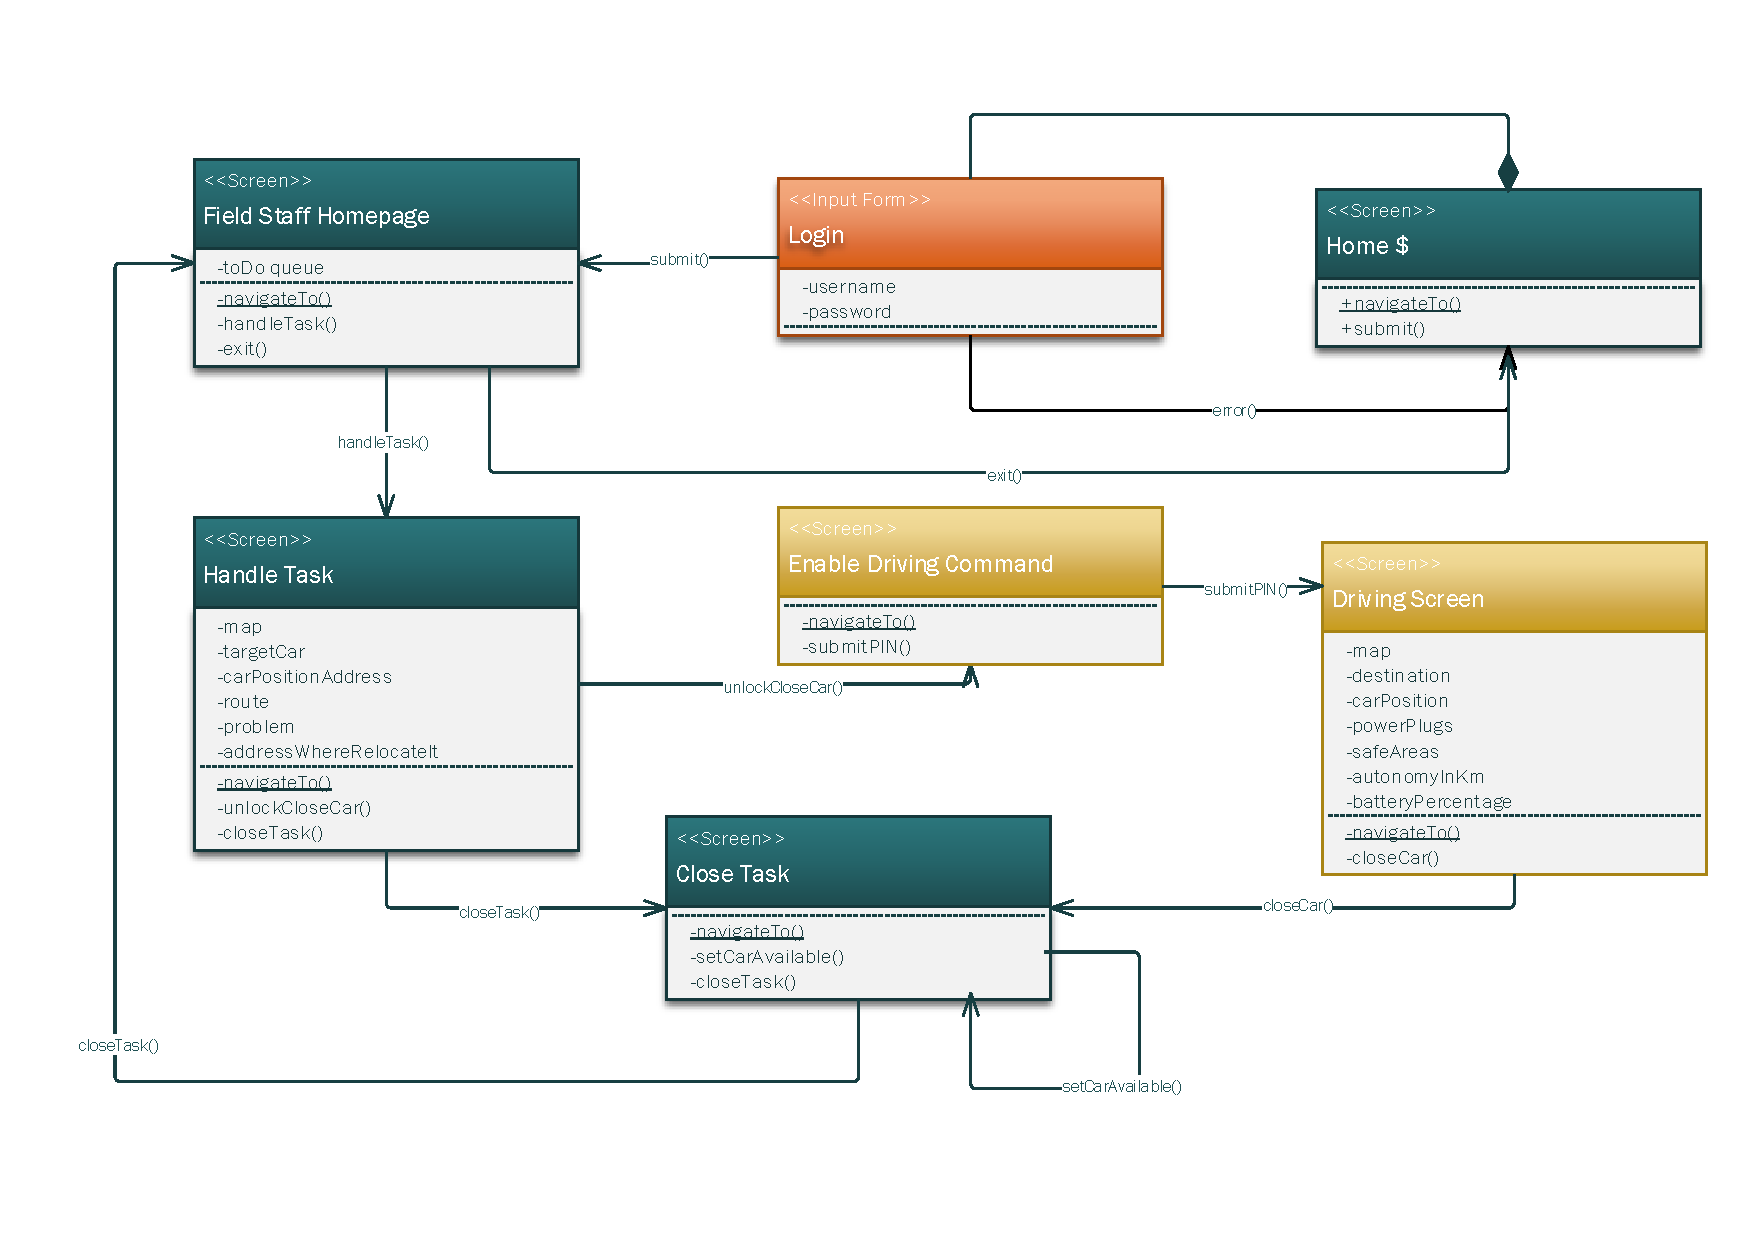
\includegraphics[scale=0.5]{./UXDiagrams/Fieldstaff/UXDiagramFieldStaffUserAuto.pdf}% "%" necessario
					\caption{Login \& Task management}
				\end{figure}
			\subsubsection{Mockups}	
				\begin{figure}[H]
					\centering
					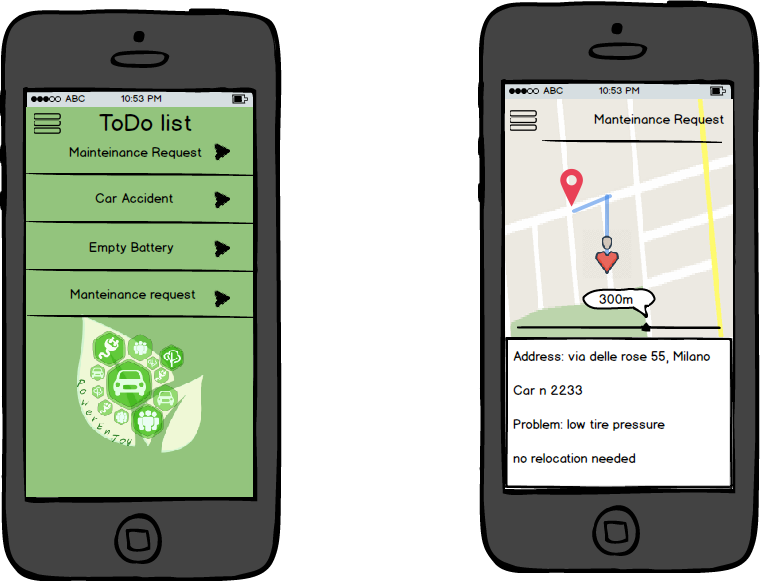
\includegraphics[scale=0.4]{./Mockups/FieldStaff/FieldStaff.png}% "%" necessario
					\caption{Car Info \& Reservation}
				\end{figure}

	\begin{landscape}
		\subsection{EmergencyStaff}
			\subsubsection{UX diagrams}
				\begin{figure}[H]
					\centering
					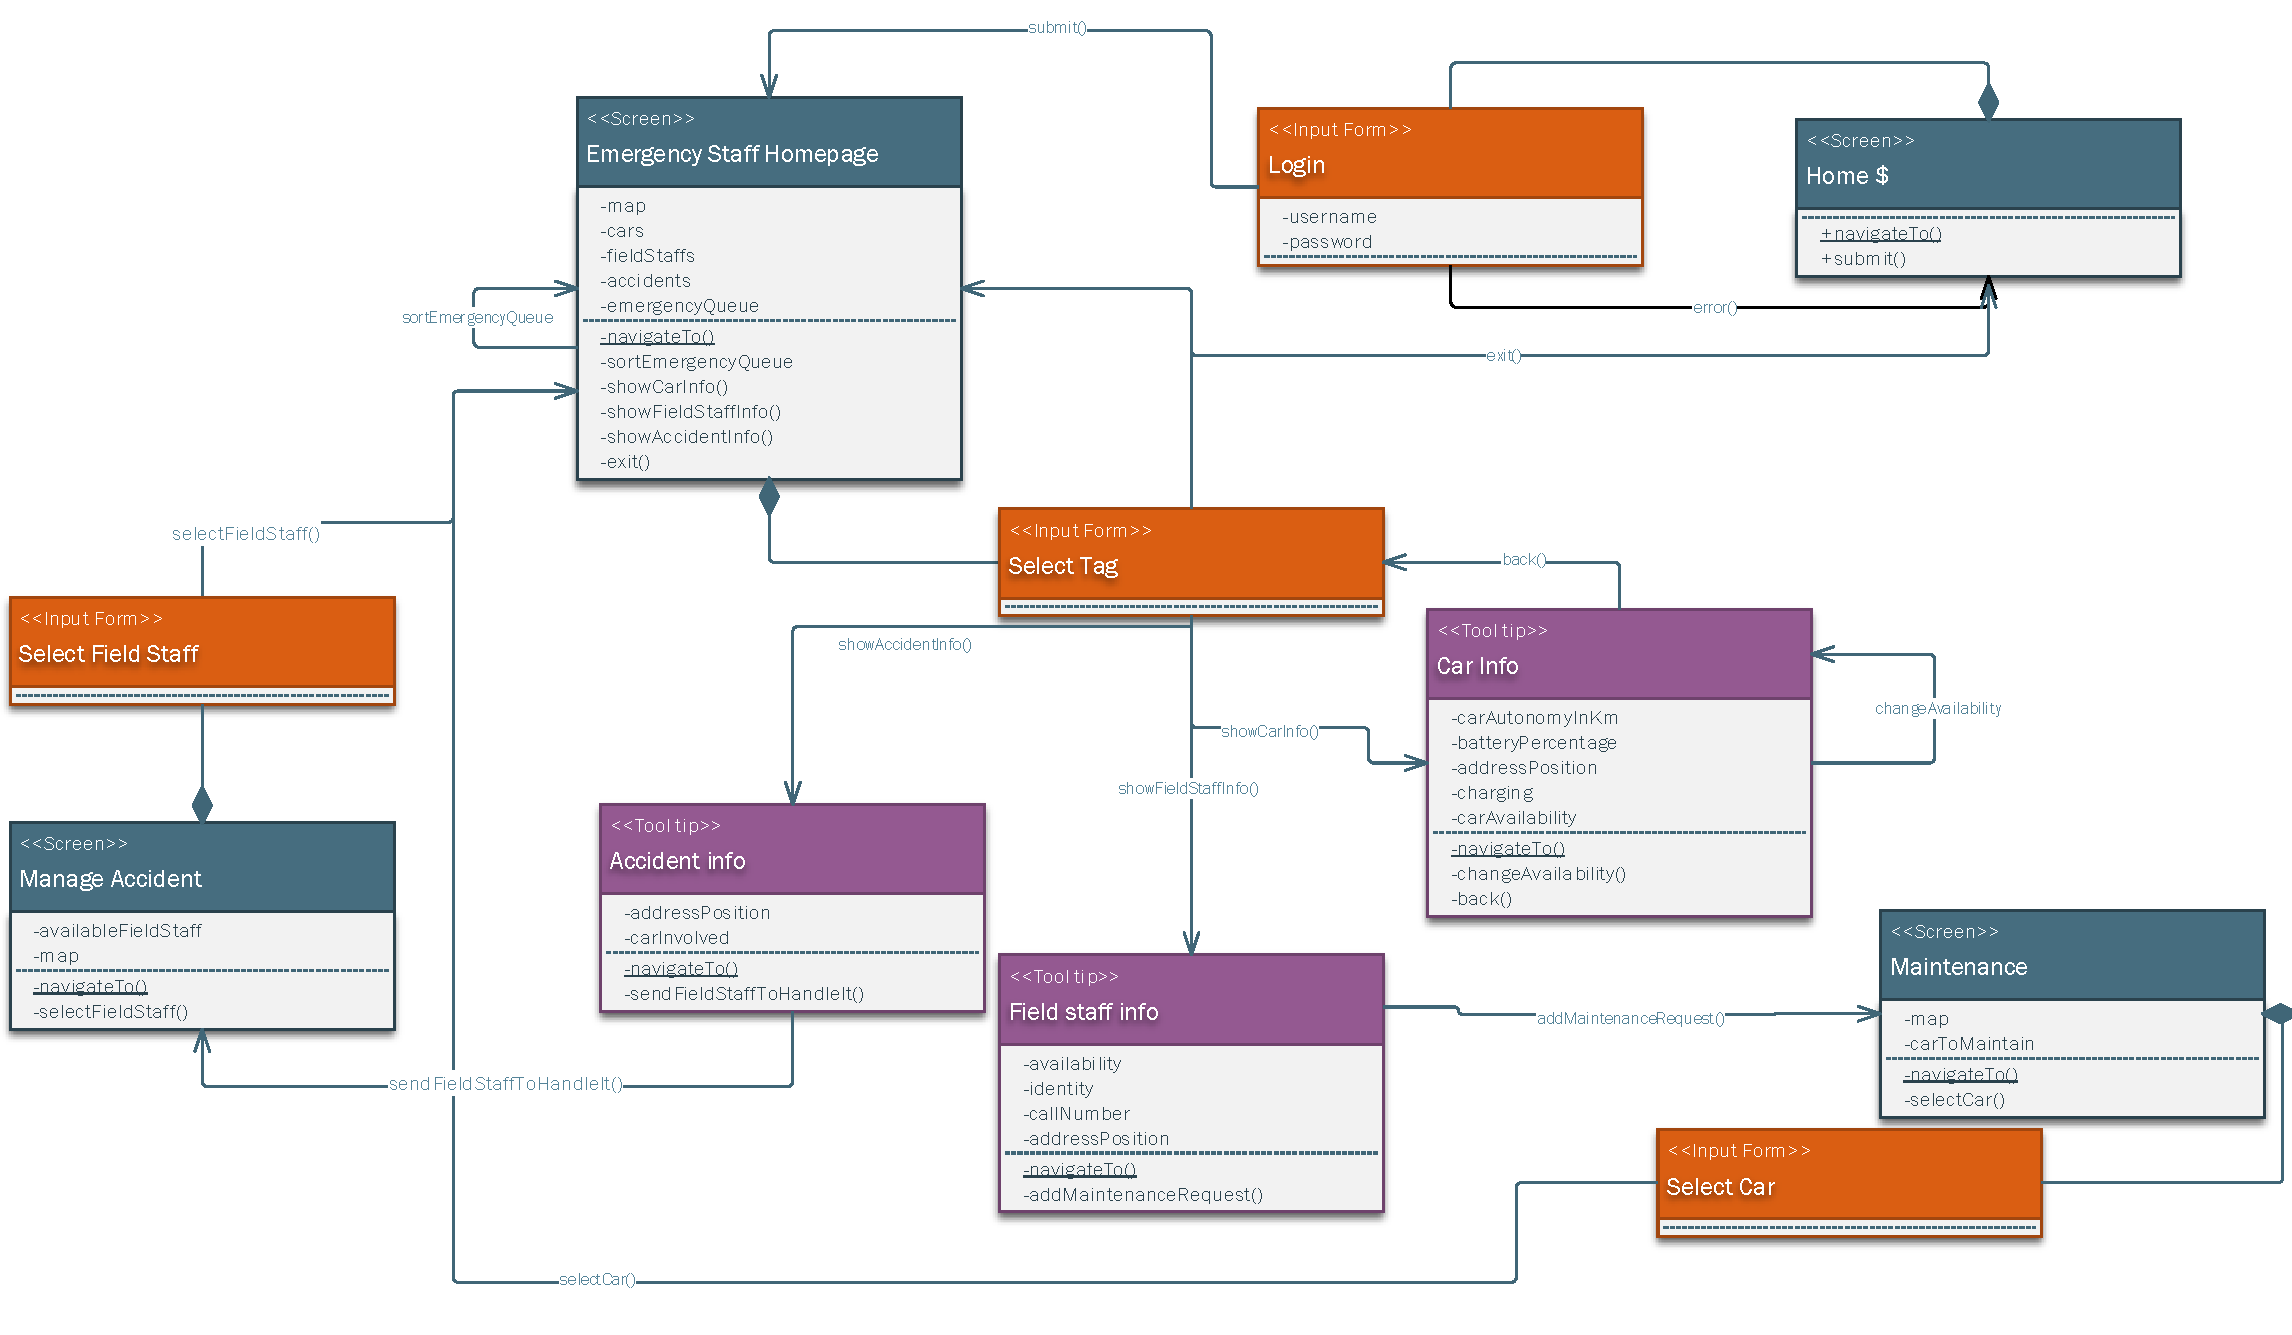
\includegraphics[scale=0.42425]{./UXDiagrams/EmergencyStaff/EmergencyStaff.pdf}% "%" necessari
					\caption{Login \& Emergency management}
				\end{figure}
	\end{landscape}
	\begin{landscape}
			\subsubsection{Mockups}
					\begin{figure}[H]
						\centering
						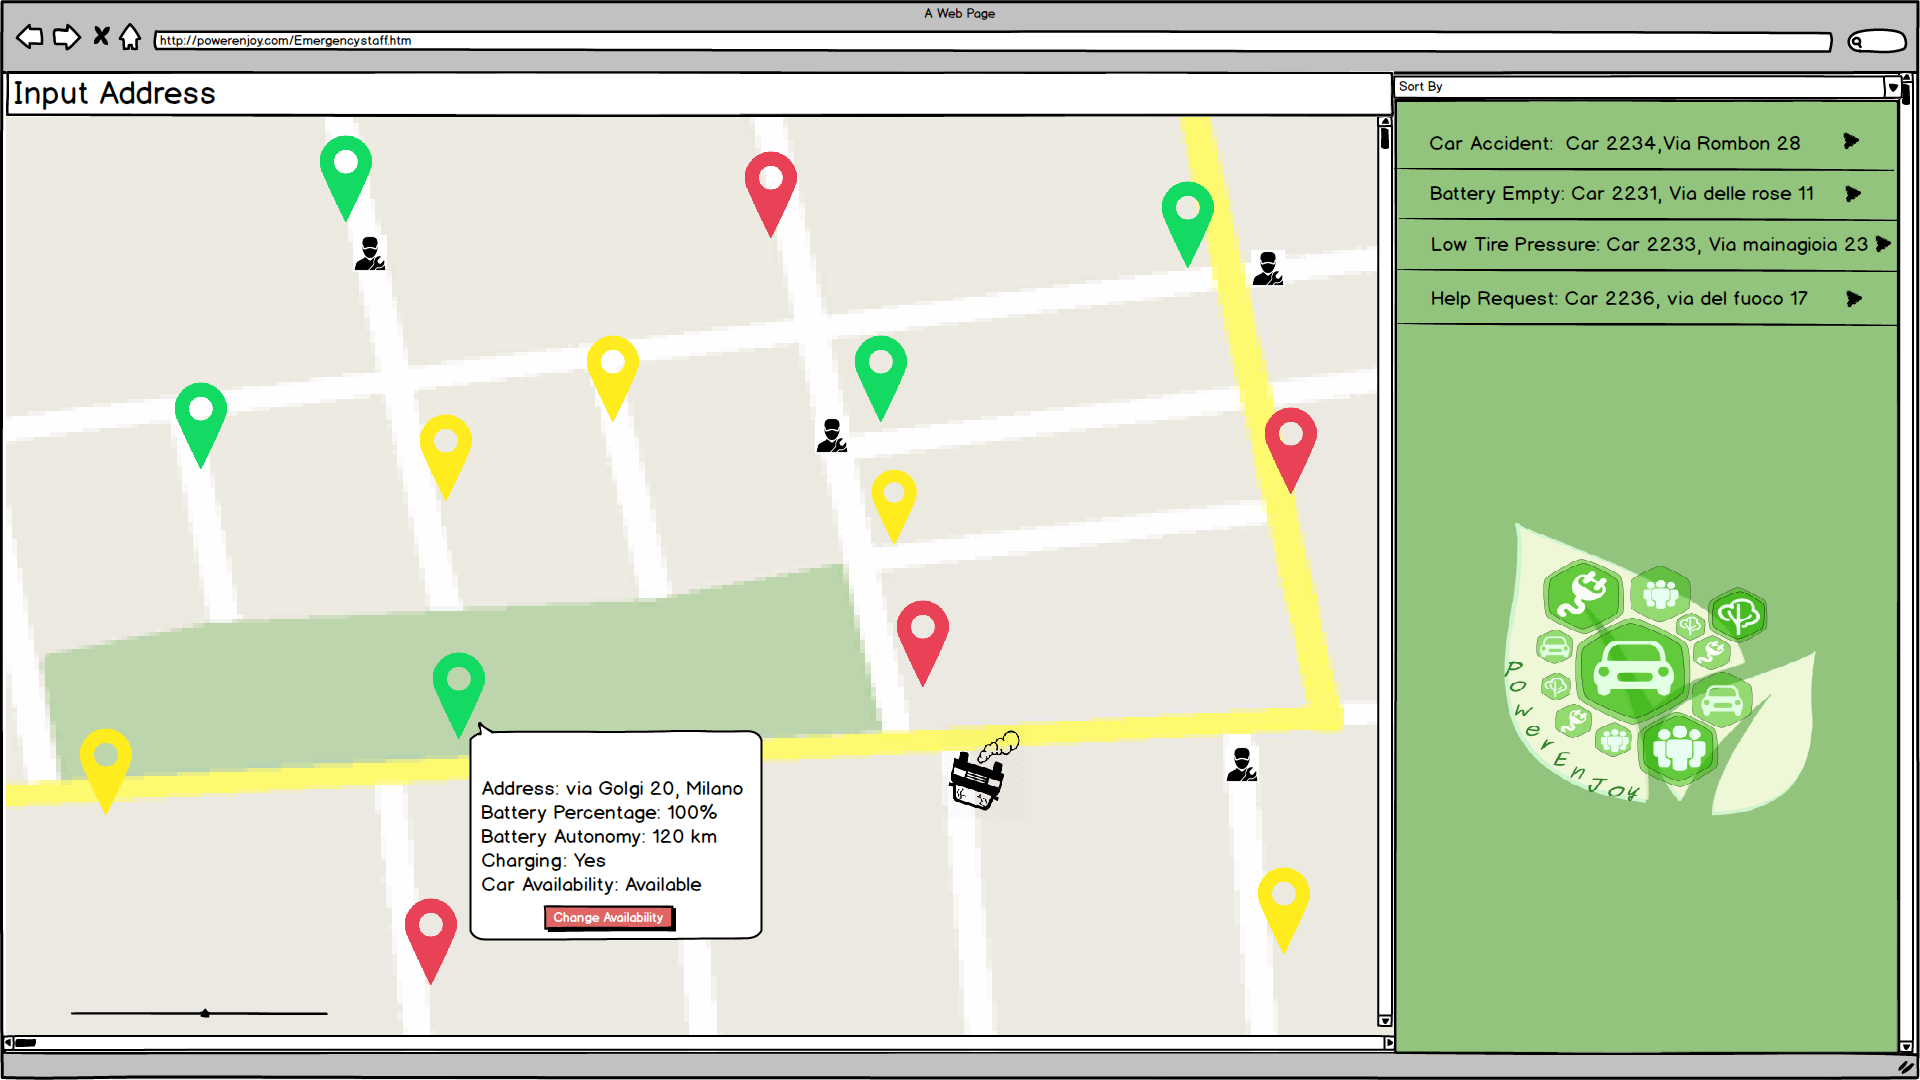
\includegraphics[scale=0.26875]{./Mockups/EmergencyStaff/EmergencyStaff.png}% "%" necessario
						\caption{Current status}
					\end{figure}
	\end{landscape}
	\begin{landscape}
	\subsection{Management Staff}
			\subsubsection{Mockup}
					\begin{figure}[H]
						\centering
						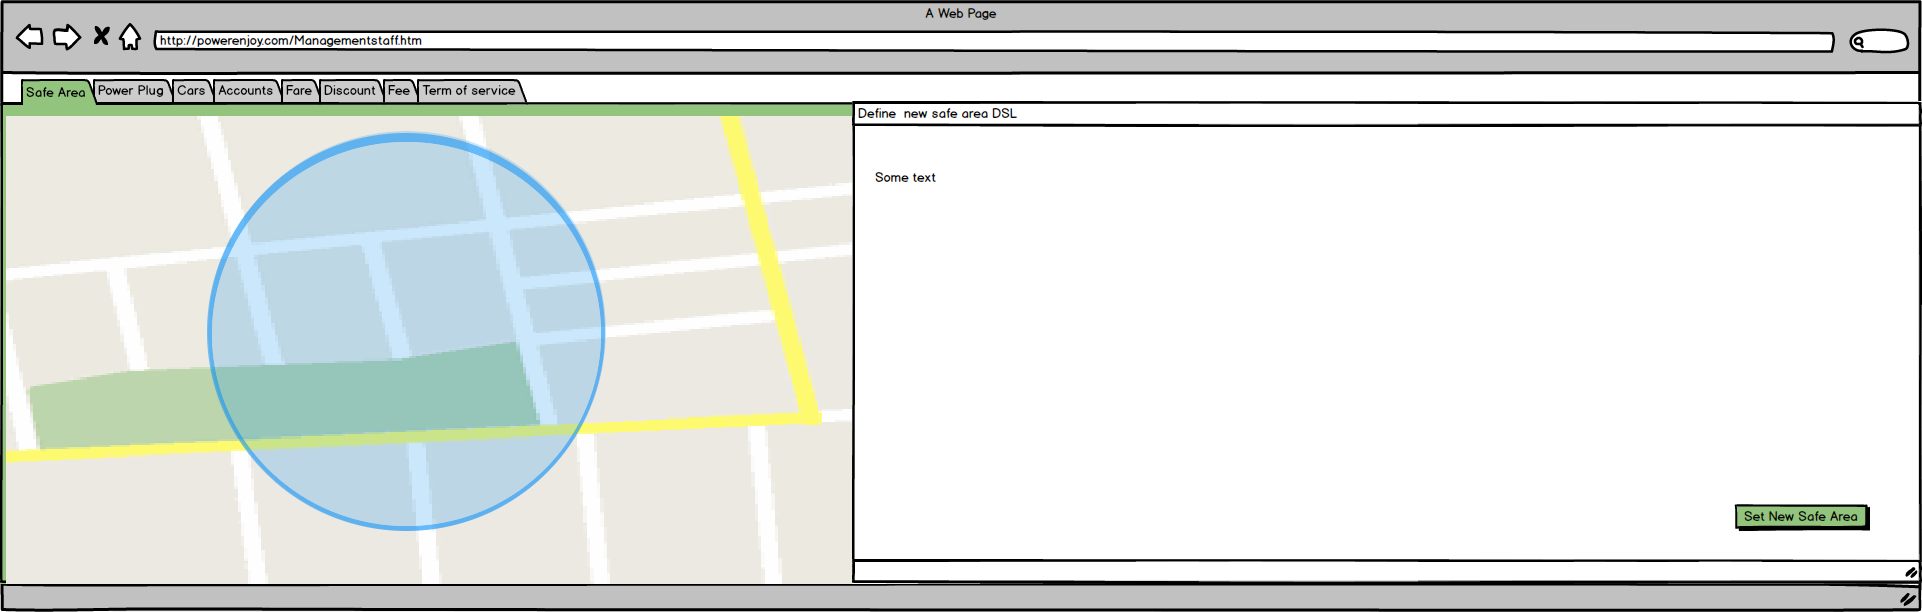
\includegraphics[scale=0.26875]{./Mockups/ManagementStaff/ManagementStaff.png}% "%" necessario
						\caption{Define a new safa area}
					\end{figure}
	\end{landscape}
	
\section{Requirements Traceability} %Explain how the requirements you have defined in the RASD map to the design elements that you have defined in this document.
\subsection{Guest User}
\begin{center}
	\begin{tabular}{|c|c|p{5cm}|} \hline
		\multirow{2}{*}{Reference} &\multirow{2}{*}{Requirements} & {Component}\\ [8px] \hline 
		\multirow{2}{*}{R.1} &\multirow{2}{*} {register to the system}&{ Account Manager }\\[8px] \hline
		\multirow{2}{*}{R.2} & \multirow{2}{*}{receive back password and PIN code }& {Account Manager }\\ [8px] \hline
	\end{tabular}
\end{center}

\subsection{Registered User}
\begin{center}
	\begin{tabular}{|c|c|p{5cm}|} \hline
		\multirow{2}{*}{Reference} &\multirow{2}{*}{Requirements} &  \multirow{2}{*}{Component}\\ [8px] \hline 
		\multirow{2}{*}{R.3} &\multirow{2}{*} {log-in}&{Account Manager }\\[8px] \hline
		\multirow{2}{*}{R.4} & \multirow{2}{*}{reset the password }&{Account Manager }\\ [8px] \hline
		\multirow{2}{*}{R.5} & \multirow{2}{*}{modify account data }& {Account Manager }\\ [8px] \hline
	\end{tabular}	
\end{center}

\subsection{PowerEnjoy User}
\begin{center}
	\begin{tabular}{|c|c|p{5cm}|} \hline
		\multirow{2}{*}{Reference} &\multirow{2}{*}{Requirements} & \multirow{2}{*}{Component}\\ [8px] \hline 
		\multirow{2}{*}{R.6} &\multirow{2}{*} {find available cars}&{Map Manager}\\[8px] \hline
		\multirow{2}{*}{R.7} & \multirow{2}{*}{reserve a car}& {Reservation Manager}\\ [8px] \hline
		\multirow{2}{*}{R.8} & \multirow{2}{*}{cancel reservation}&{Reservation Manager}\\ [8px] \hline
		\multirow{2}{*}{R.9} & \multirow{2}{*}{to be charged of a fee}&{Reservation manager, Payment Manager}\\ [8px] \hline
		\multirow{2}{*}{R.10} & \multirow{2}{*}{to rent a car}&{Rent Manager}\\ [8px] \hline
		\multirow{2}{*}{R.11} & \multirow{2}{*}{to be excluded from the fruition of PowerEnjoy services} &{Account Manager, Management Staff Manager}\\ [8px] \hline
		\multirow{2}{*}{R.12...15} & \multirow{2}{*}{Discounts}& {Rent Manager, Service configuration}\\ [8px] \hline
		\multirow{2}{*}{R.16} & \multirow{2}{*}{enable the money saving option}& {BPM, Map Manager, Google Maps API, Car App, Car Manager}\\ [8px] \hline
		\multirow{2}{*}{R.17} & \multirow{2}{*}{notified of changes in the service policies}& {Management Staff Manager, Push Notification Adapter, PowerEnjoy WebApp, PowerEnjoy User Manager}\\ [8px] \hline
	\end{tabular}	
\end{center}

\subsection{Field Staff users}
	\begin{center}
	\begin{tabular}{|c|c|p{5cm}|} \hline
		\multirow{2}{*}{Reference} &\multirow{2}{*}{Requirements} & \multirow{2}{*}{Component}\\ [8px] \hline 
		\multirow{2}{*}{R.18} &\multirow{2}{*} {To be notified of new relocation/maintenance request }&{ Field Staff App, BPM, Emergency Management, Field Staff Manager}\\[8px] \hline
		\multirow{2}{*}{R.19} & \multirow{2}{*}{relocate assigned cars}& {Car Manager,  Field Staff Manager, Field Staff App }\\ [8px] \hline
	\end{tabular}	
\end{center}

\subsection{Management Staff User}
	\begin{center}
	\begin{tabular}{|c|c|p{5cm}|} \hline
		\multirow{2}{*}{Reference} &\multirow{2}{*}{Requirements} &  \multirow{2}{*}{Component}\\ [8px] \hline 
		\multirow{2}{*}{R.21..23} &\multirow{2}{*} {Configuration}&{Management Staff Manager, Management staff Web App, Service Configurator}\\[8px] \hline
		\multirow{2}{*}{R.24} & \multirow{2}{*}{manage accounts }& {Management Staff Manager, Management staff Web, Account Manager}\\ [8px] \hline
		\multirow{2}{*}{R.25} & \multirow{2}{*}{Handle unpaid rents }& {Payement Manager, Management Staff Manager, Management staff Web, Account Manager }\\ [8px] \hline		
	\end{tabular}	
\end{center}

\subsection{Emergency Staff Users}
	\begin{center}
	\begin{tabular}{|c|c|p{5cm}|} \hline
		\multirow{2}{*}{Reference} &\multirow{2}{*}{Requirements} &  \multirow{2}{*}{Component}\\ [8px] \hline 
		\multirow{2}{*}{R.26..29} &\multirow{2}{*} {Emergency Management}&{Emergency Manager, Emergency Staff Manager, Emergency Staff Web App}\\[8px] \hline	
	\end{tabular}	
\end{center}

\subsection{Third Party Developers}
	\begin{center}
	\begin{tabular}{|c|c|p{5cm}|} \hline
		\multirow{2}{*}{Reference} &\multirow{2}{*}{Requirements} &  \multirow{2}{*}{Component}\\ [8px] \hline 
		\multirow{2}{*}{R.30..31} &\multirow{2}{*} {API Access}&{External App Manager}\\[8px] \hline
	\end{tabular}	
\end{center}

\subsection{General Purpose Requirements}
	\begin{center}
	\begin{tabular}{|c|c|p{5cm}|} \hline
		\multirow{2}{*}{Reference} &\multirow{2}{*}{Requirements} &  \multirow{2}{*}{Component}\\ [8px] \hline 
		\multirow{2}{*}{R.32} &\multirow{2}{*} {No multiple rent/reservation from the same user}&{Rent/Reservation Managers}\\[8px] \hline	
		\multirow{2}{*}{R.33} &\multirow{2}{*} {Car Unavailable when accident occurs}&{Car Manager, Car App}\\[8px] \hline	
		\multirow{2}{*}{R.34} &\multirow{2}{*} {Car Relocation is canceled if an accident occurs}&{BPM, Car Manager, Car App}\\[8px] \hline
		\multirow{2}{*}{R.35} &\multirow{2}{*} {Last Busy Field staff work assignment}&{BPM, Emergency Manager}\\[8px] \hline	
	\end{tabular}	
	
\end{center}

\clearpage
\section{Effort Spent} %In this section you will include information about the number of hours each group member  has worked towards the fulfillment of this deadline.
	\begin{itemize}
		\item Alessandro Erba $\approx$ 43h
		\item Filippo Leveni 	$\approx$ 43h
		\item Luca Lodi $\approx$ 43h
	\end{itemize}
\section{References}
\end{document}